\documentclass[11pt,a4paper]{article}

\usepackage[margin=2.2cm]{geometry}
\usepackage{amsmath,amssymb}
\usepackage{graphicx}
\usepackage{subcaption}
\usepackage{booktabs}
\usepackage{float}
\usepackage{enumitem}
\usepackage[hidelinks]{hyperref}
\usepackage{caption}

\captionsetup{font=small,labelfont=bf}
\graphicspath{{Q1/}{Q2/}}
\setlength{\parskip}{0.5em}
\setlength{\parindent}{0pt}

\begin{document}

% ---------------------------------------------------------------------
% Title page
% ---------------------------------------------------------------------
\begin{titlepage}
    \centering
    \vspace*{3cm}
    {\large Department of Electronic and Telecommunication Engineering\\
    University of Moratuwa, Sri Lanka\par}
    \vspace{3cm}
    {\LARGE\bfseries BM4152 Biosignal Processing\par}
    \vspace{0.8cm}
    {\Large Assignment 3\par}
    \vspace{0.4cm}
    {\Large Continuous and Discrete Wavelet Transforms\par}
    \vspace{4cm}
    {\large
    \begin{tabular}{ll}
        Name:         & M. I. Nadha \\
        Index Number: & 220409J
    \end{tabular}\par}
    \vfill
    {\large \today\par}
\end{titlepage}

\tableofcontents
\newpage

% =====================================================================
\section{Continuous Wavelet Transform}
% =====================================================================

The continuous wavelet transform (CWT) analyses a signal by correlating it with scaled and translated copies of a mother wavelet, giving a joint time--scale representation suited to non-stationary signals. In this section the normalized Mexican-hat wavelet is derived, its properties are verified, and it is used to decompose a signal whose frequency changes with time.

\subsection{Wavelet properties}

\subsubsection*{(i) Derivation of the Mexican-hat function}

With $\mu = 0$ and $\sigma = 1$ the Gaussian is
\begin{equation}
    g(t) = \frac{1}{\sqrt{2\pi}}\, e^{-t^2/2}.
\end{equation}
Differentiating twice,
\begin{align}
    \frac{d}{dt} g(t)     &= -t\, g(t), \\
    \frac{d^2}{dt^2} g(t) &= -g(t) + t^2 g(t) = (t^2 - 1)\, g(t),
\end{align}
so that
\begin{equation}
    m(t) = -\frac{d^2}{dt^2} g(t) = \frac{1}{\sqrt{2\pi}}\,(1 - t^2)\, e^{-t^2/2}.
\end{equation}

\subsubsection*{(ii) Normalizing factor}

The energy of $m(t)$ is
\begin{equation}
    E = \int_{-\infty}^{\infty} m^2(t)\,dt
      = \frac{1}{2\pi}\int_{-\infty}^{\infty} \left(1 - 2t^2 + t^4\right) e^{-t^2}\,dt .
\end{equation}
Using the standard Gaussian integrals
$\int e^{-t^2}dt = \sqrt{\pi}$,
$\int t^2 e^{-t^2}dt = \tfrac{\sqrt{\pi}}{2}$ and
$\int t^4 e^{-t^2}dt = \tfrac{3\sqrt{\pi}}{4}$,
\begin{equation}
    E = \frac{1}{2\pi}\left(\sqrt{\pi} - \sqrt{\pi} + \frac{3\sqrt{\pi}}{4}\right)
      = \frac{3}{8\sqrt{\pi}} \approx 0.2116 .
\end{equation}
For unit energy, $m(t)$ must be multiplied by
\begin{equation}
    c = \frac{1}{\sqrt{E}} = \sqrt{\frac{8\sqrt{\pi}}{3}} \approx 2.174 .
\end{equation}

\subsubsection*{(iii) Normalized mother and daughter wavelets}

\begin{equation}
    \psi(t) = c\, m(t) = \frac{2}{\sqrt{3}\,\pi^{1/4}}\,(1 - t^2)\, e^{-t^2/2},
    \qquad \frac{2}{\sqrt{3}\,\pi^{1/4}} \approx 0.8673 .
\end{equation}
Including the scale $s$ and the translation $\tau$, the generic daughter wavelet is
\begin{equation}
    \psi_{s,\tau}(t) = \frac{1}{\sqrt{s}}\,\psi\!\left(\frac{t-\tau}{s}\right)
    = \frac{2}{\sqrt{3s}\,\pi^{1/4}}
      \left[1 - \left(\frac{t-\tau}{s}\right)^{2}\right]
      \exp\!\left[-\frac{1}{2}\left(\frac{t-\tau}{s}\right)^{2}\right].
\end{equation}
The factor $1/\sqrt{s}$ keeps the energy of every daughter wavelet equal to that of the mother wavelet.

\subsubsection*{(iv) Time-domain daughter wavelets}

The function \texttt{mexican\_hat(t, scale, translation)} of the provided script was completed with the expression above and evaluated for the 20 scales $s = 0.01, 0.11, \dots, 1.91$ on the time axis $t = n/f_s$, $n = -3000,\dots,3000$, $f_s = 250$~Hz. Figure~\ref{fig:daughters} shows each wavelet zoomed to its own support and Figure~\ref{fig:daughters_overlay} shows all of them on a common axis.

\begin{figure}[H]
    \centering
    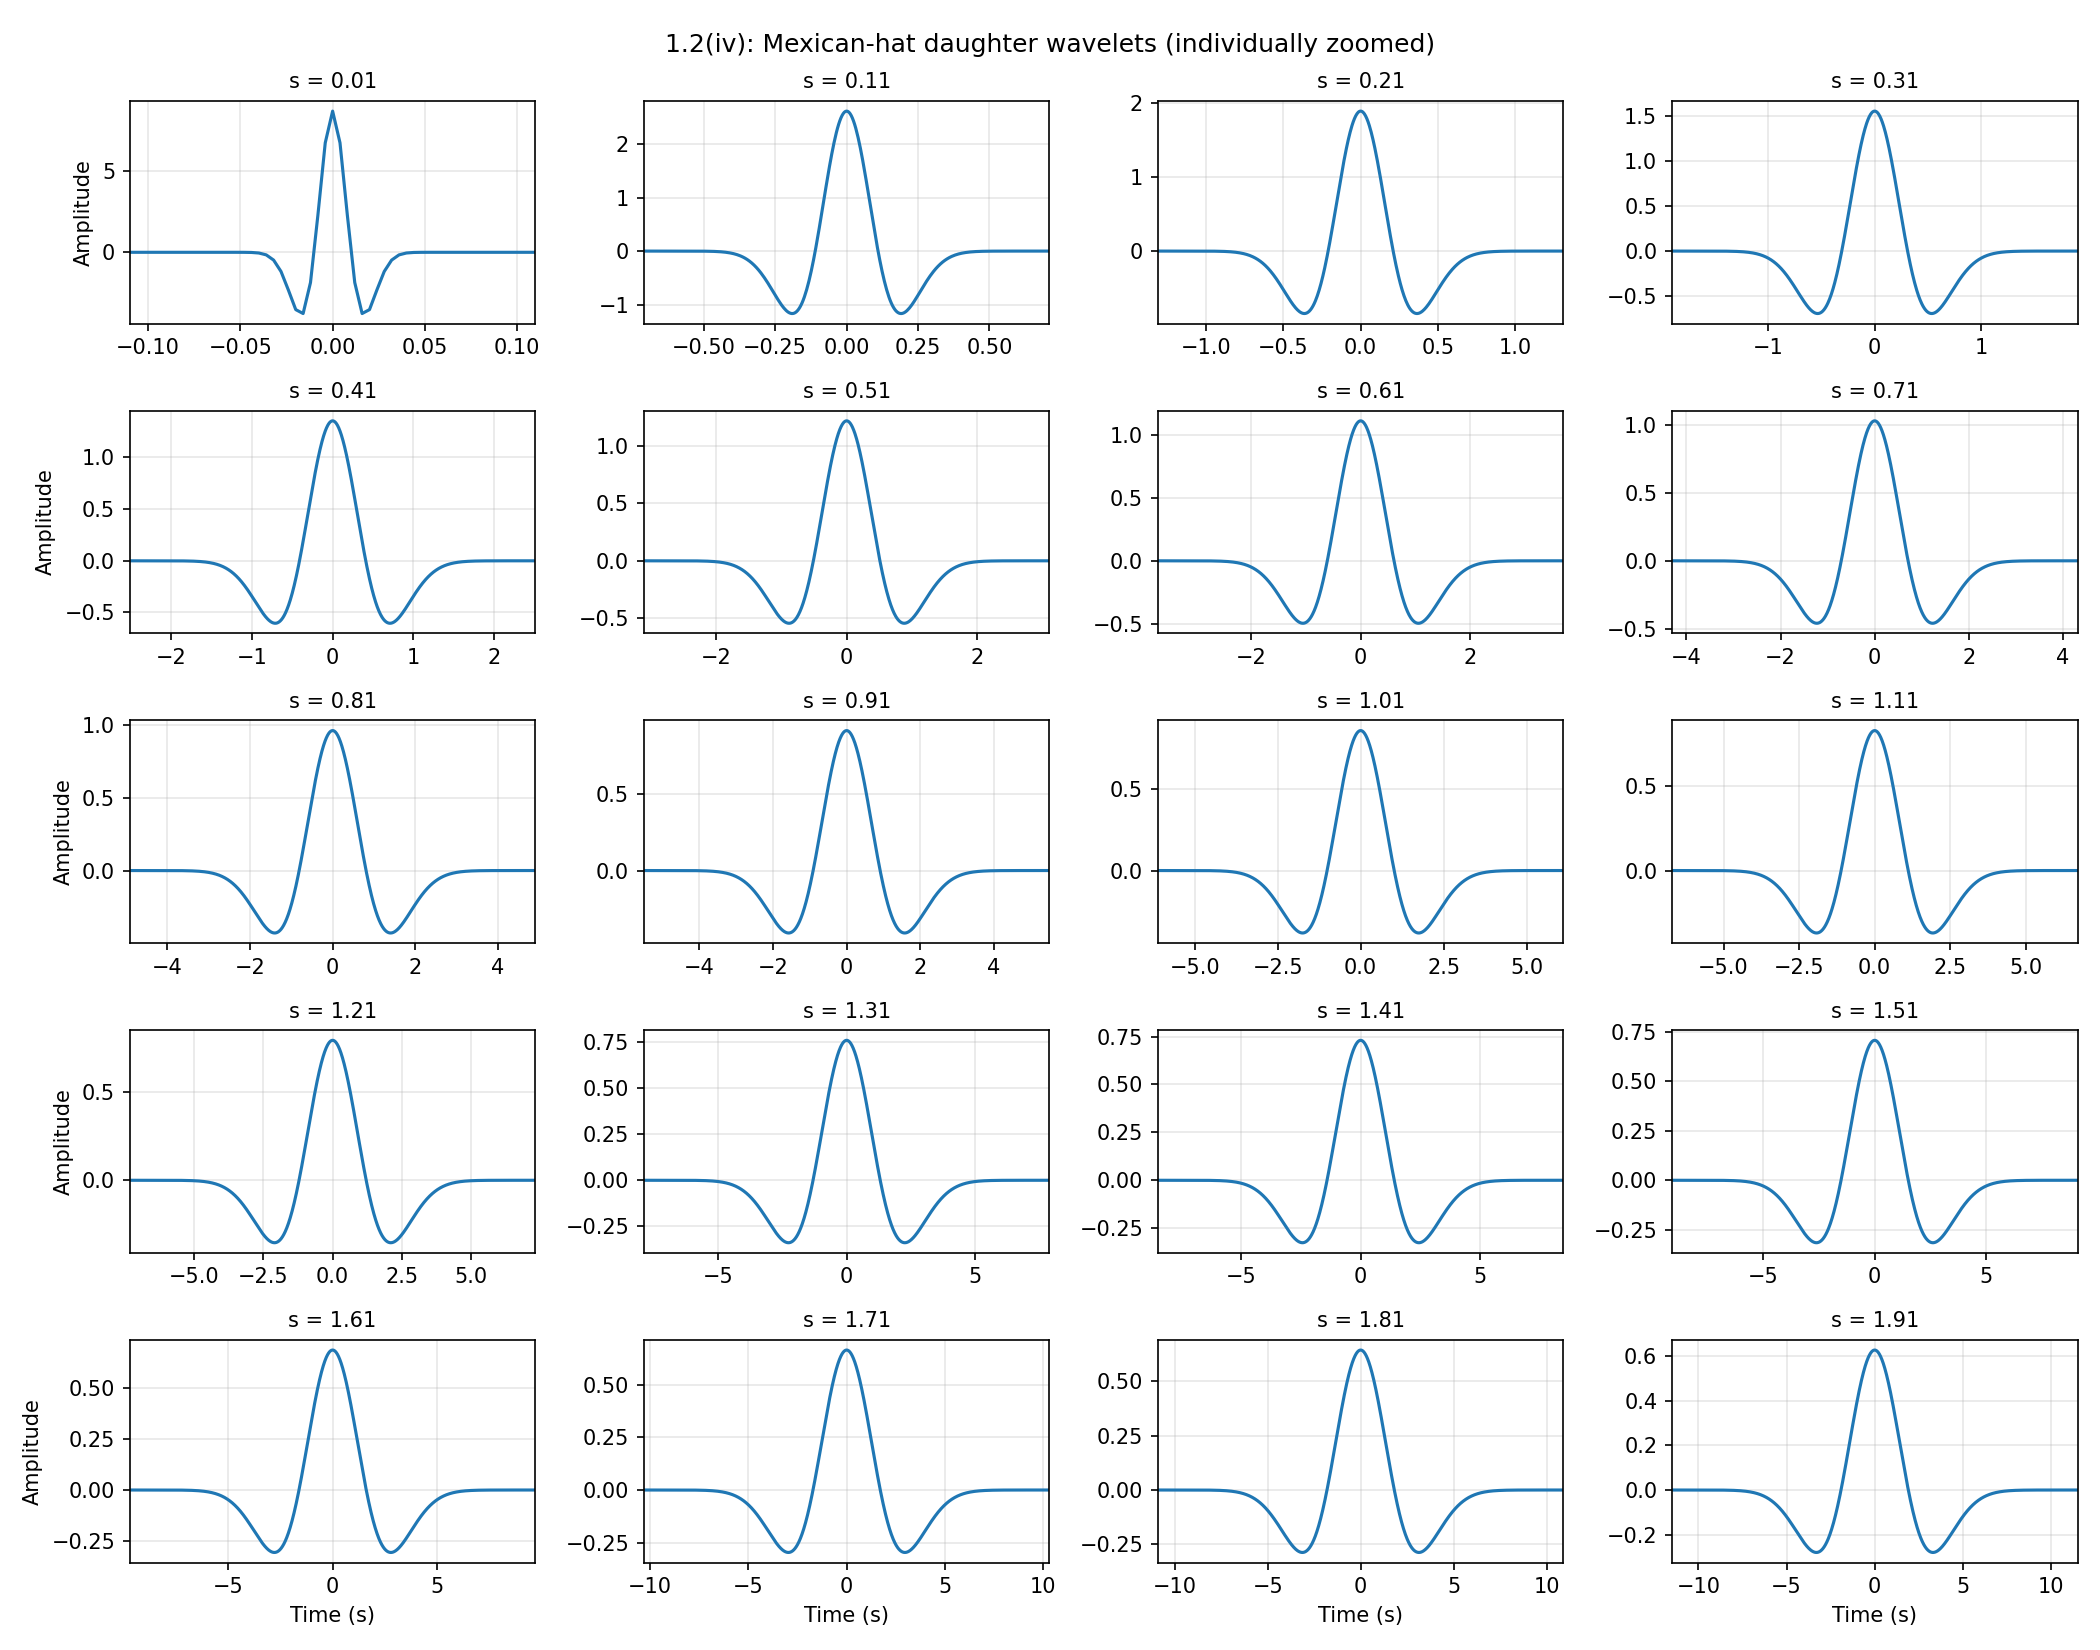
\includegraphics[width=0.95\textwidth]{fig1_2_iv_daughter_wavelets.png}
    \caption{Mexican-hat daughter wavelets for $s = 0.01 + 0.1k$, $k = 0,\dots,19$ (each panel zoomed to $\pm 6s$).}
    \label{fig:daughters}
\end{figure}

\begin{figure}[H]
    \centering
    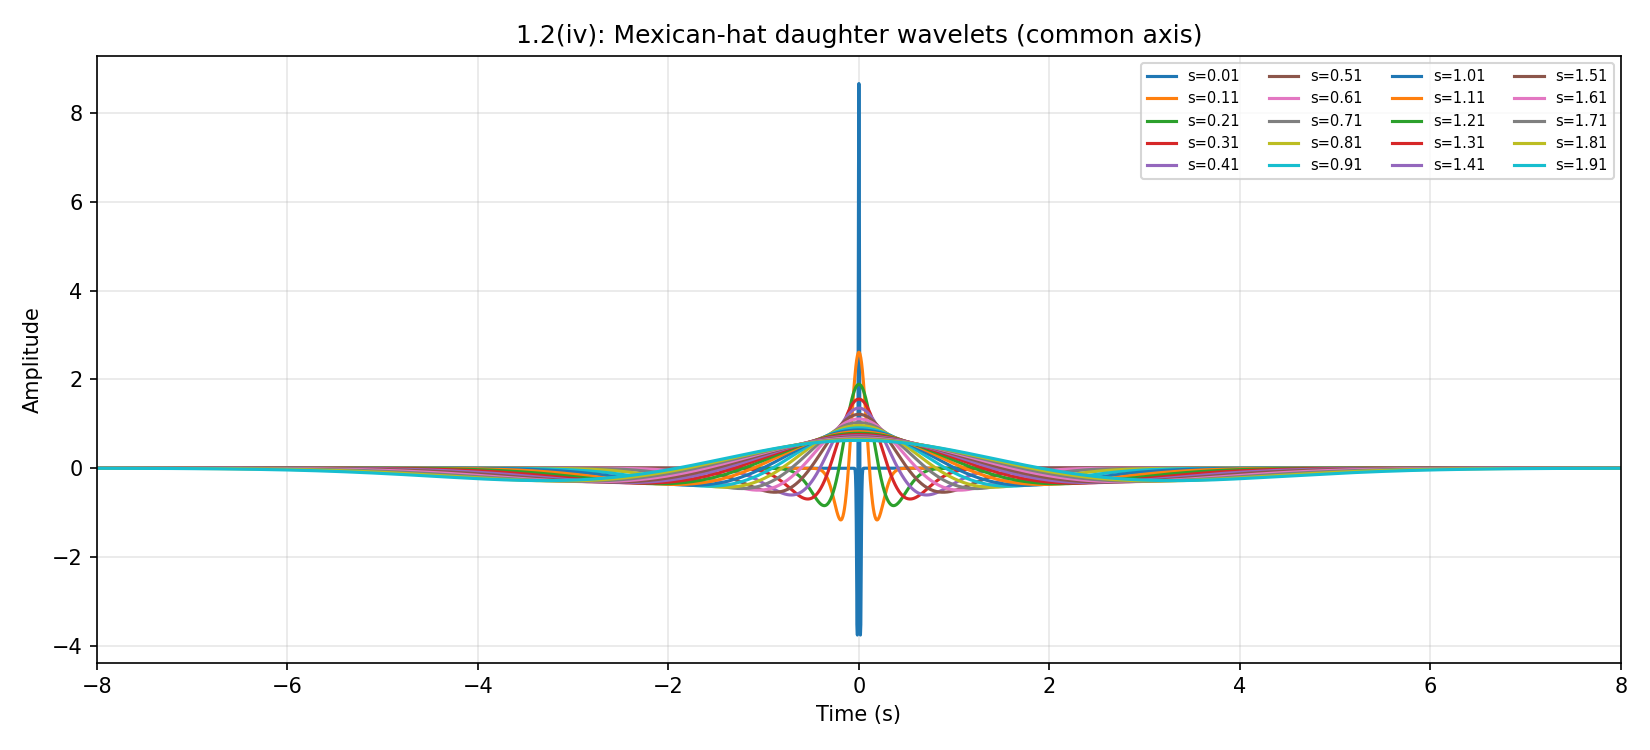
\includegraphics[width=0.85\textwidth]{fig1_2_iv_daughter_wavelets_overlay.png}
    \caption{The same daughter wavelets on a common time axis.}
    \label{fig:daughters_overlay}
\end{figure}

All daughter wavelets have the same shape. As the scale increases the wavelet is stretched in time and, because of the $1/\sqrt{s}$ factor, its peak amplitude decreases as $0.8673/\sqrt{s}$. Small scales give narrow, tall wavelets and large scales give wide, low wavelets.

\subsubsection*{(v) Verification of wavelet properties}

The mean $\int\psi_s(t)\,dt$ and the energy $\int\psi_s^2(t)\,dt$ were evaluated numerically (sum multiplied by $\Delta t = 1/f_s$). The effective support was measured as the width of the region in which $|\psi_s(t)|$ exceeds $0.1\%$ of its peak. The results are given in Table~\ref{tab:props} and Figure~\ref{fig:props}.

\begin{table}[H]
    \centering
    \small
    \begin{tabular}{cccc@{\hspace{1.2cm}}cccc}
        \toprule
        $s$ & Mean & Energy & Support (s) & $s$ & Mean & Energy & Support (s) \\
        \midrule
        0.01 & $-2.5\times10^{-17}$ & 1.000000 & 0.088 & 1.01 & $6.8\times10^{-17}$  & 1.000000 & 8.952 \\
        0.11 & $6.2\times10^{-18}$  & 1.000000 & 0.968 & 1.11 & $-4.9\times10^{-18}$ & 1.000000 & 9.840 \\
        0.21 & $-3.9\times10^{-17}$ & 1.000000 & 1.856 & 1.21 & $-1.1\times10^{-17}$ & 1.000000 & 10.728 \\
        0.31 & $-4.7\times10^{-17}$ & 1.000000 & 2.744 & 1.31 & $1.1\times10^{-16}$  & 1.000000 & 11.616 \\
        0.41 & $2.4\times10^{-17}$  & 1.000000 & 3.632 & 1.41 & $3.2\times10^{-15}$  & 1.000000 & 12.504 \\
        0.51 & $5.0\times10^{-17}$  & 1.000000 & 4.520 & 1.51 & $3.2\times10^{-13}$  & 1.000000 & 13.392 \\
        0.61 & $-3.4\times10^{-17}$ & 1.000000 & 5.408 & 1.61 & $1.4\times10^{-11}$  & 1.000000 & 14.280 \\
        0.71 & $2.2\times10^{-18}$  & 1.000000 & 6.296 & 1.71 & $3.2\times10^{-10}$  & 1.000000 & 15.160 \\
        0.81 & $5.7\times10^{-17}$  & 1.000000 & 7.184 & 1.81 & $4.4\times10^{-9}$   & 1.000000 & 16.048 \\
        0.91 & $2.8\times10^{-17}$  & 1.000000 & 8.064 & 1.91 & $4.0\times10^{-8}$   & 1.000000 & 16.936 \\
        \bottomrule
    \end{tabular}
    \caption{Numerically evaluated mean, energy and effective support of the daughter wavelets.}
    \label{tab:props}
\end{table}

\begin{figure}[H]
    \centering
    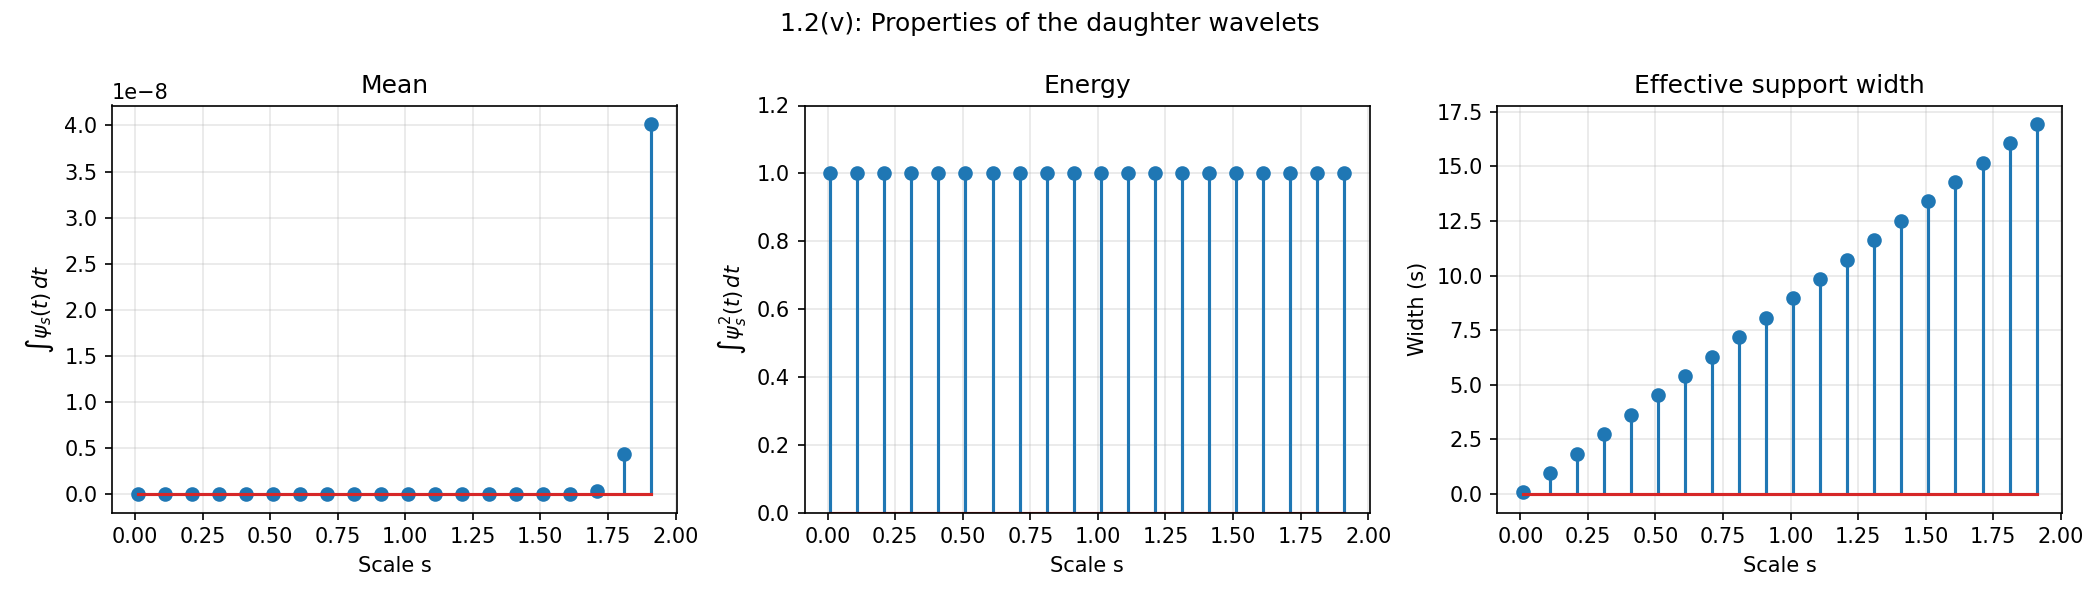
\includegraphics[width=0.95\textwidth]{fig1_2_v_wavelet_properties.png}
    \caption{Mean, energy and effective support width of the daughter wavelets against scale.}
    \label{fig:props}
\end{figure}

\begin{itemize}[leftmargin=*]
    \item \textbf{Zero mean:} the mean of every daughter wavelet is numerically zero. For most scales it is at the level of floating-point round-off ($\sim10^{-17}$). For the largest scales it rises to about $10^{-8}$ because the tails of the widest wavelets are slightly truncated by the finite $\pm12$~s time window; this is still negligible. Zero mean is the admissibility condition: the wavelet has no DC component and behaves as a band-pass filter.
    \item \textbf{Unit energy:} the energy is $1.000000$ for all scales, which confirms the normalizing factor derived in part (ii) and the $1/\sqrt{s}$ scaling.
    \item \textbf{Compact support:} the Mexican hat is not strictly compactly supported because the Gaussian envelope never reaches exactly zero, but it decays so rapidly that the wavelet is effectively confined to about $\pm 4.4s$. The effective support grows linearly with scale (approximately $8.9s$), so each wavelet is well localized in time.
\end{itemize}

\subsubsection*{(vi) Spectra of the daughter wavelets}

\begin{figure}[H]
    \centering
    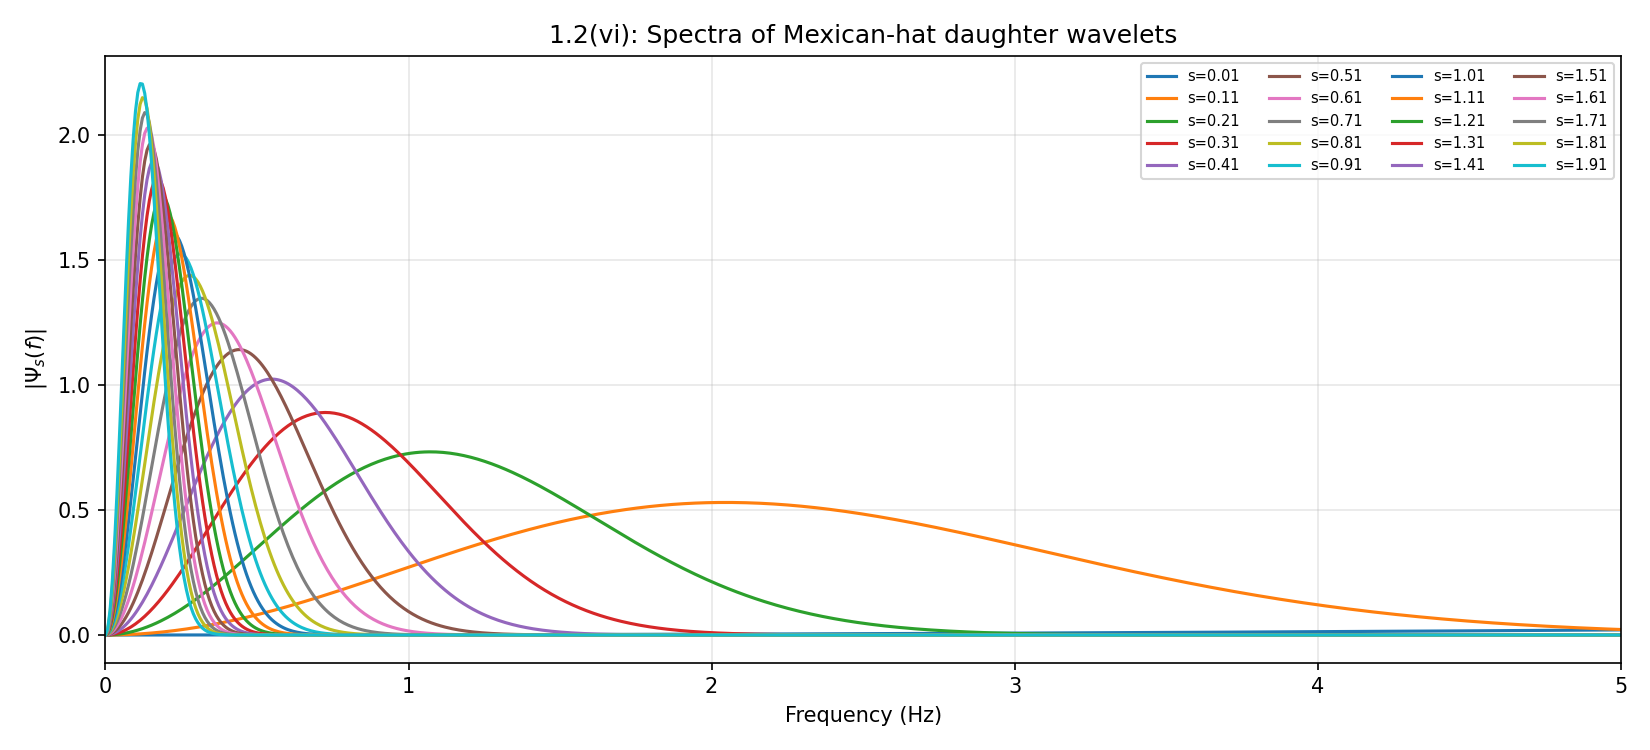
\includegraphics[width=0.9\textwidth]{fig1_2_vi_wavelet_spectra.png}
    \caption{Magnitude spectra of the daughter wavelets (linear frequency axis).}
    \label{fig:spectra}
\end{figure}

\begin{figure}[H]
    \centering
    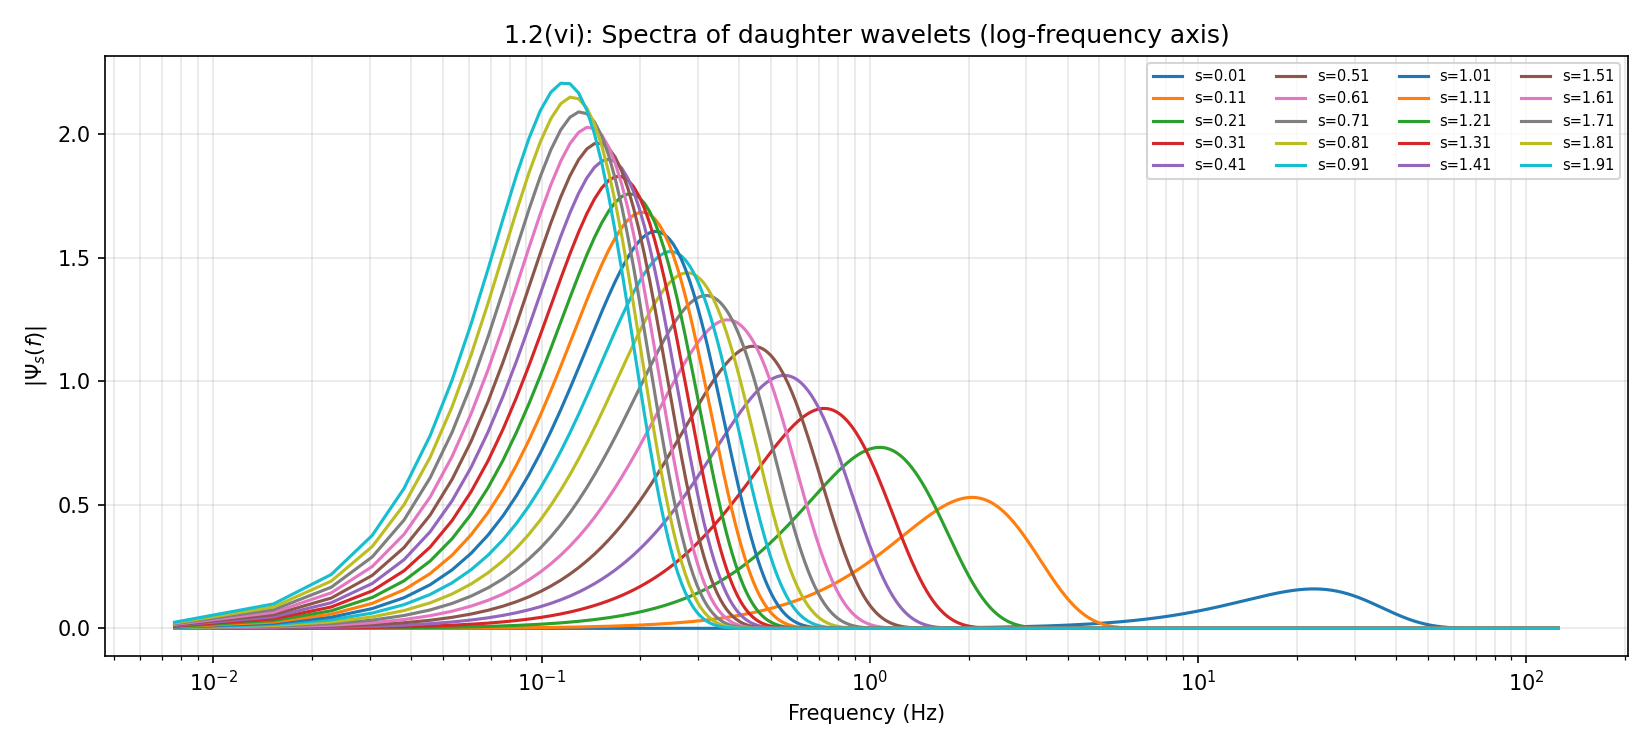
\includegraphics[width=0.9\textwidth]{fig1_2_vi_wavelet_spectra_log.png}
    \caption{Magnitude spectra of the daughter wavelets on a logarithmic frequency axis.}
    \label{fig:spectra_log}
\end{figure}

The Fourier transform of the daughter wavelet is $\Psi_s(f) = \sqrt{s}\,\Psi(sf)$ with $|\Psi(f)| \propto f^2 e^{-(2\pi f)^2/2}$. The following observations can be made from Figures~\ref{fig:spectra} and~\ref{fig:spectra_log}.

\begin{itemize}[leftmargin=*]
    \item Every spectrum is zero at $f = 0$ (consistent with the zero-mean property) and decays to zero at high frequencies, so each daughter wavelet is a \textbf{band-pass filter}.
    \item The centre frequency is inversely proportional to the scale, $f_c = \sqrt{2}/(2\pi s)$. The measured peak frequencies agree with this expression for every scale; for example $s = 0.11$ gives 2.045~Hz (theory 2.046~Hz), $s = 1.01$ gives 0.221~Hz (theory 0.223~Hz) and $s = 0.01$ gives 22.5~Hz, which lies outside the plotted range.
    \item The bandwidth is also inversely proportional to the scale. Small scales give wide bands at high frequency (good time resolution, poor frequency resolution) and large scales give narrow bands at low frequency (good frequency resolution, poor time resolution). On the logarithmic axis all spectra have the same shape and are merely shifted, which shows that the ratio of centre frequency to bandwidth is constant (\textbf{constant-Q} filter bank).
    \item The peak magnitude grows as $\sqrt{s}$ since the same unit energy is concentrated in a narrower band.
\end{itemize}

\subsection{Continuous wavelet decomposition}

\subsubsection*{(i) Test signal}

The signal $x[n]$ was created with $N = 3000$ and $f_s = 250$~Hz. It contains a 0.25~Hz sinusoid for $1 \le n < 4500$ and a 0.75~Hz sinusoid for $4500 \le n < 9000$ (Figure~\ref{fig:cwt_signal}).

\begin{figure}[H]
    \centering
    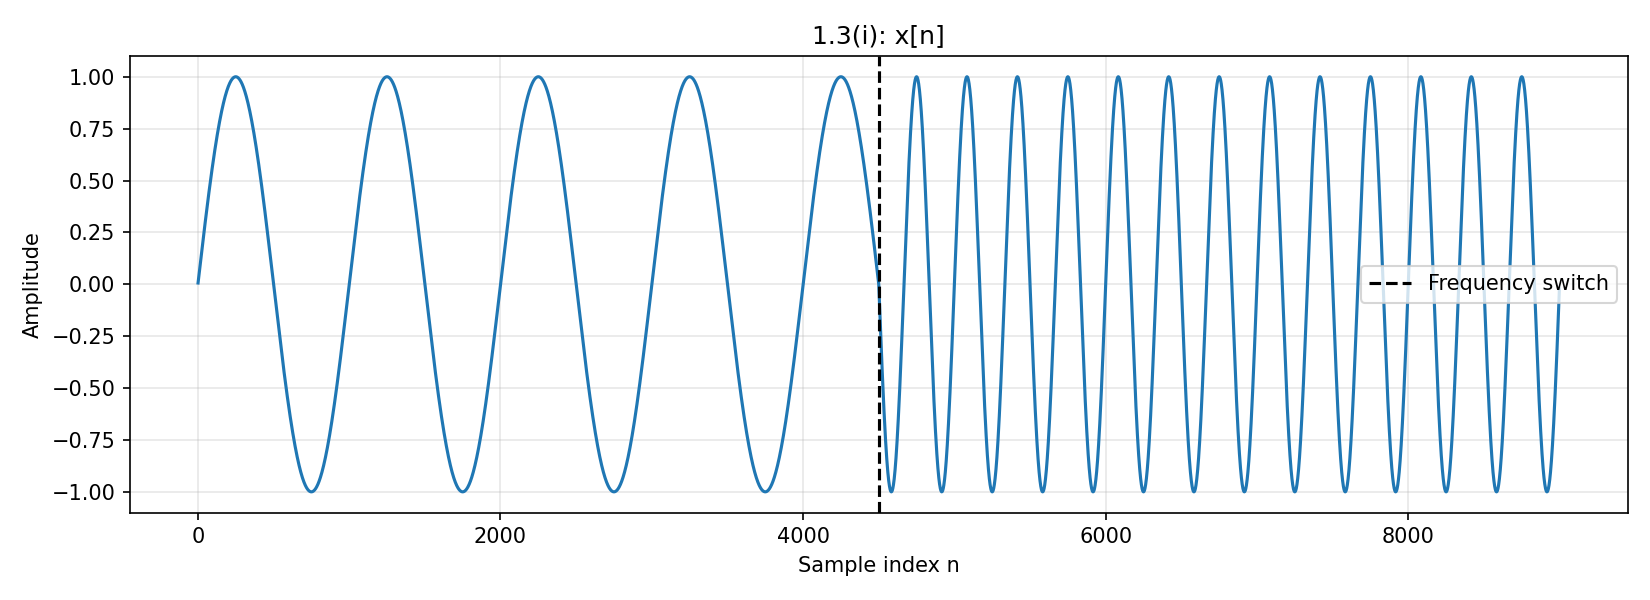
\includegraphics[width=0.85\textwidth]{fig1_3_i_signal.png}
    \caption{Non-stationary test signal $x[n]$.}
    \label{fig:cwt_signal}
\end{figure}

\subsubsection*{(ii)--(iii) CWT and spectrogram}

For each of the 200 scales $s = 0.01, 0.02, \dots, 2.00$ the signal was convolved with the corresponding daughter wavelet using \texttt{scipy.signal.fftconvolve(x, wavelet, mode='same')}, and the result was multiplied by $\Delta t$ to approximate the CWT integral. Since the Mexican hat is an even function, convolution is identical to the correlation required by the CWT definition, and each sample of the output corresponds to one translation $\tau$. Each convolution gives one row of the $200 \times 8999$ coefficient matrix. All 200 rows are plotted together in Figure~\ref{fig:cwt_rows}, coloured by scale, and the complete matrix is displayed with \texttt{pcolormesh} in Figure~\ref{fig:cwt}.

\begin{figure}[H]
    \centering
    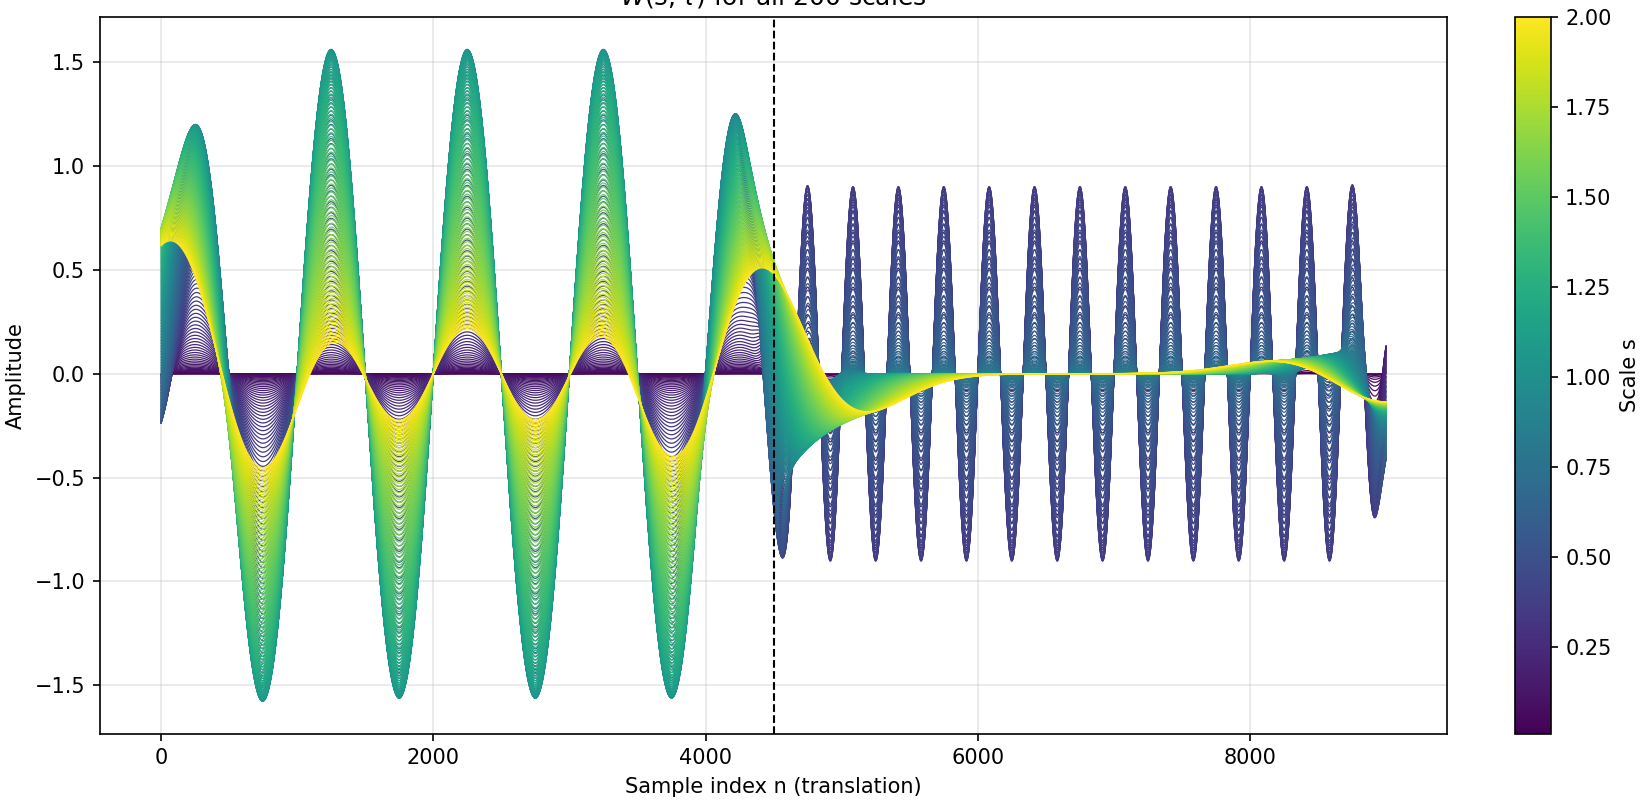
\includegraphics[width=0.9\textwidth]{fig1_3_ii_cwt_all_scales.png}
    \caption{$x[n]$ and its CWT coefficients $W(s,\tau)$ for all 200 scales; each line is the convolution output at one scale.}
    \label{fig:cwt_rows}
\end{figure}

Each scale acts as a band-pass filter on the signal. During the 0.25~Hz segment the largest outputs (amplitude about 1.55) come from scales near $s = 1$, while the smallest scales give almost no output. During the 0.75~Hz segment the largest outputs (amplitude about 0.9) come from small scales near $s = 0.3$, and the large scales decay to zero shortly after the transition at $n = 4500$. Every output oscillates at the frequency of the signal segment it responds to.

\begin{figure}[H]
    \centering
    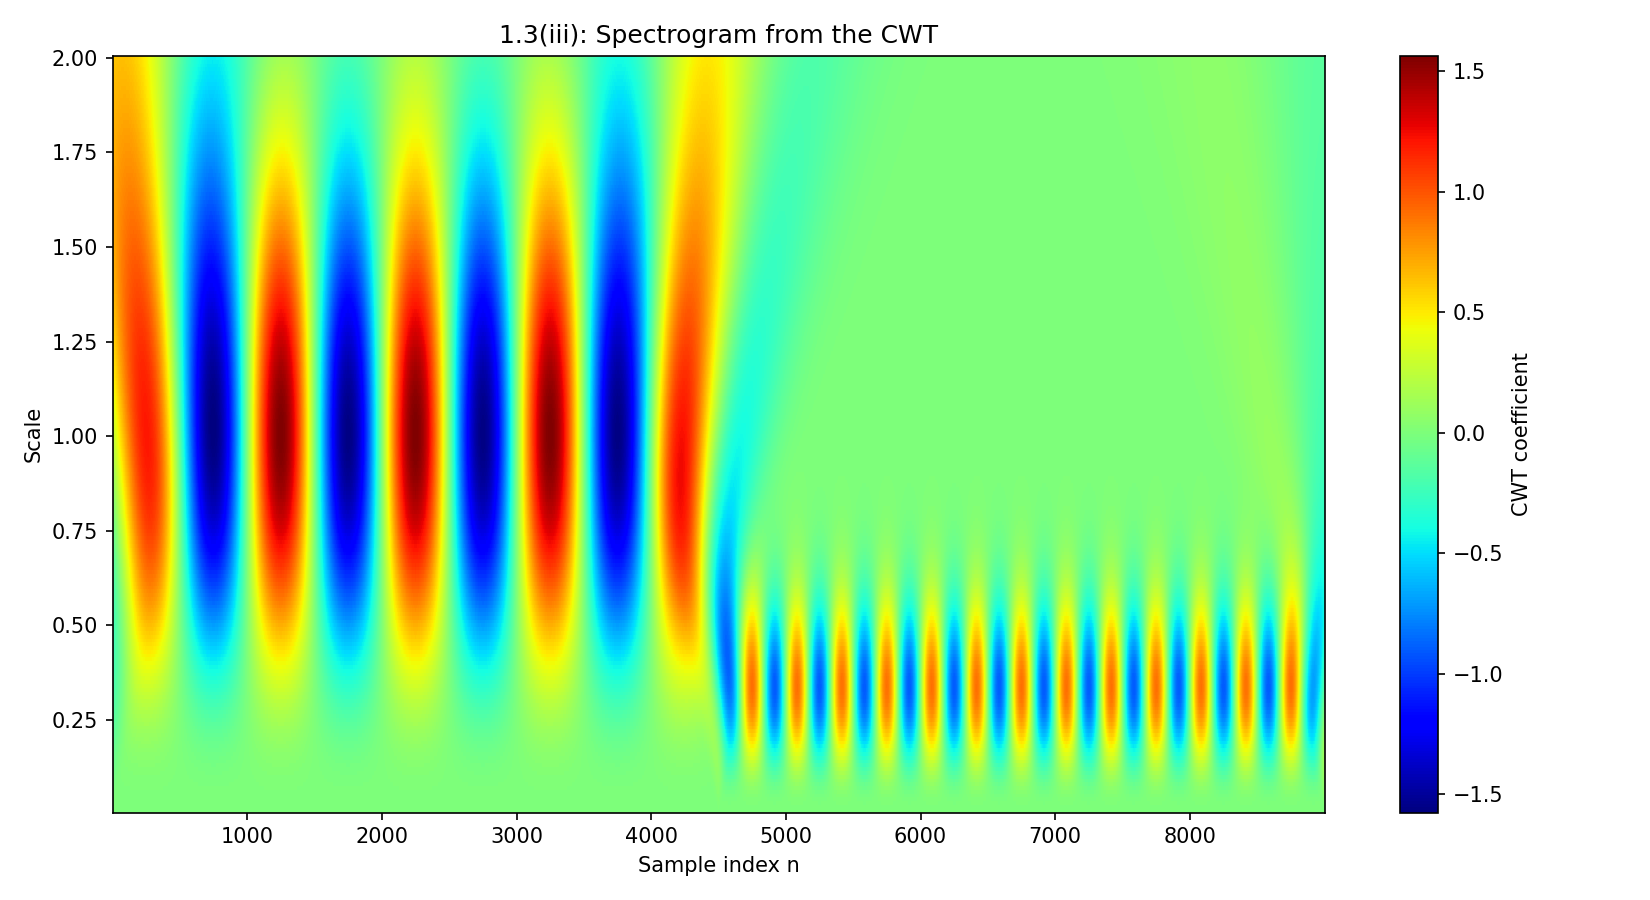
\includegraphics[width=0.95\textwidth]{fig1_3_iii_cwt_spectrogram.png}
    \caption{Spectrogram (scalogram) of $x[n]$ obtained from the CWT.}
    \label{fig:cwt}
\end{figure}

\begin{figure}[H]
    \centering
    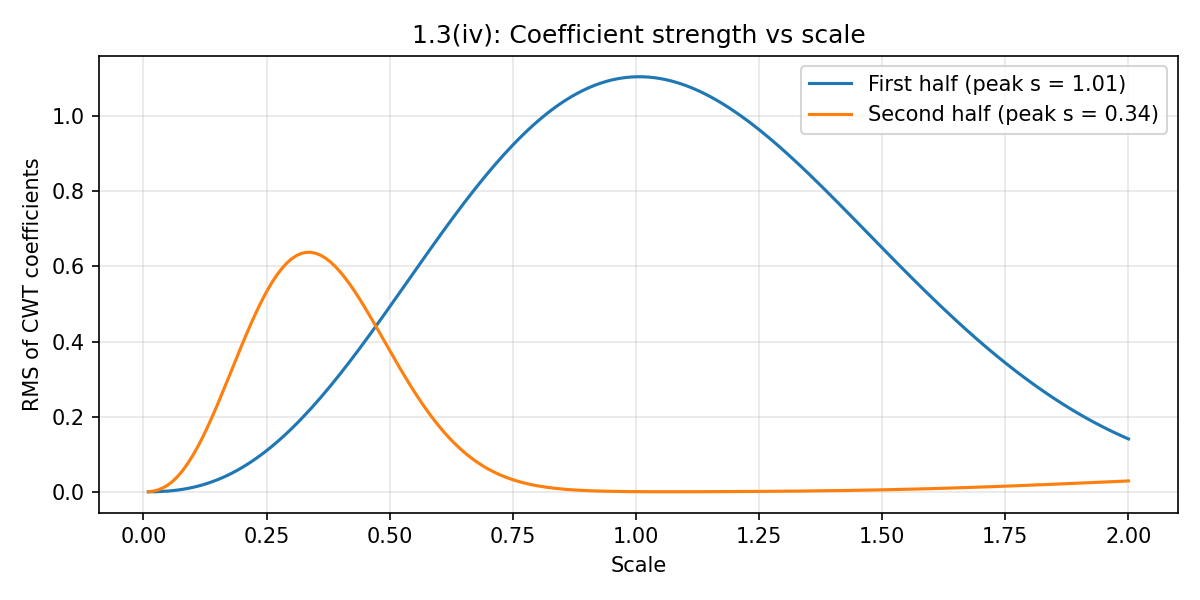
\includegraphics[width=0.7\textwidth]{fig1_3_iv_rms_vs_scale.png}
    \caption{RMS value of the CWT coefficients against scale for each half of the signal.}
    \label{fig:cwt_rms}
\end{figure}

\subsubsection*{(iv) Discussion}

\begin{itemize}[leftmargin=*]
    \item \textbf{Frequency is mapped to scale.} In the first half of the signal the coefficients are large in a band centred near $s \approx 1.0$, whereas in the second half the energy moves to a band centred near $s \approx 0.34$. The low-frequency component (0.25~Hz) matches a stretched wavelet and the higher-frequency component (0.75~Hz) matches a compressed wavelet, which is the expected inverse relationship between scale and frequency.
    \item \textbf{The scale ratio equals the frequency ratio.} For a sinusoid of frequency $f$ the coefficient amplitude is proportional to $\sqrt{s}\,|\Psi(sf)| \propto s^{5/2} e^{-(2\pi f s)^2/2}$, which is maximum at $s = \sqrt{5/2}/(2\pi f)$. This predicts $s = 1.007$ for 0.25~Hz and $s = 0.336$ for 0.75~Hz. The measured maxima in Figure~\ref{fig:cwt_rms} are $s = 1.01$ and $s = 0.34$, and their ratio is 3, the same as the ratio of the two frequencies.
    \item \textbf{Time localization.} The change of frequency is clearly located at $n = 4500$. A Fourier transform of the whole signal would show two spectral peaks but give no information about when each frequency occurs.
    \item \textbf{Oscillating coefficients.} The Mexican hat is a real wavelet, so the coefficients oscillate between positive and negative values at the frequency of the signal. The stripes are therefore wide in the first half and three times narrower in the second half.
    \item \textbf{Time--frequency trade-off.} At large scales the wavelets are long, so the transition at $n = 4500$ is smeared over a wide region, while at small scales the transition is sharp. The band of the 0.25~Hz component is also much wider along the scale axis than that of the 0.75~Hz component, which follows from the constant-Q behaviour.
    \item \textbf{Edge effects.} Near $n = 0$ and $n = 9000$ the wavelets extend beyond the signal, which is implicitly zero-padded by the convolution. The coefficients in these regions are distorted, more so at large scales (cone of influence).
\end{itemize}

% =====================================================================
\section{Discrete Wavelet Transform}
% =====================================================================

The discrete wavelet transform (DWT) removes the redundancy of the CWT by using dyadic scales and translations, implemented efficiently as a filter bank that splits the signal into approximation and detail sub-bands. In this section the DWT is applied with the db9 and Haar wavelets using PyWavelets, and is then used to denoise two synthetic signals and to compress an ECG recording.

\subsection{Applying the DWT with PyWavelets}

\subsubsection*{(i) Test signals}

The signals $x_1[n]$ (a sum of sinusoids whose frequencies change at $n = 512$) and $x_2[n]$ (a piecewise-constant signal) were created with $f_s = 512$~Hz and 1024 samples. Both were corrupted with additive white Gaussian noise at 10~dB SNR using the provided \texttt{awgn} helper with a fixed random seed, giving $y_1[n]$ and $y_2[n]$ (Figure~\ref{fig:signals}). The same stored noisy signals were used for both wavelets throughout.

\begin{figure}[H]
    \centering
    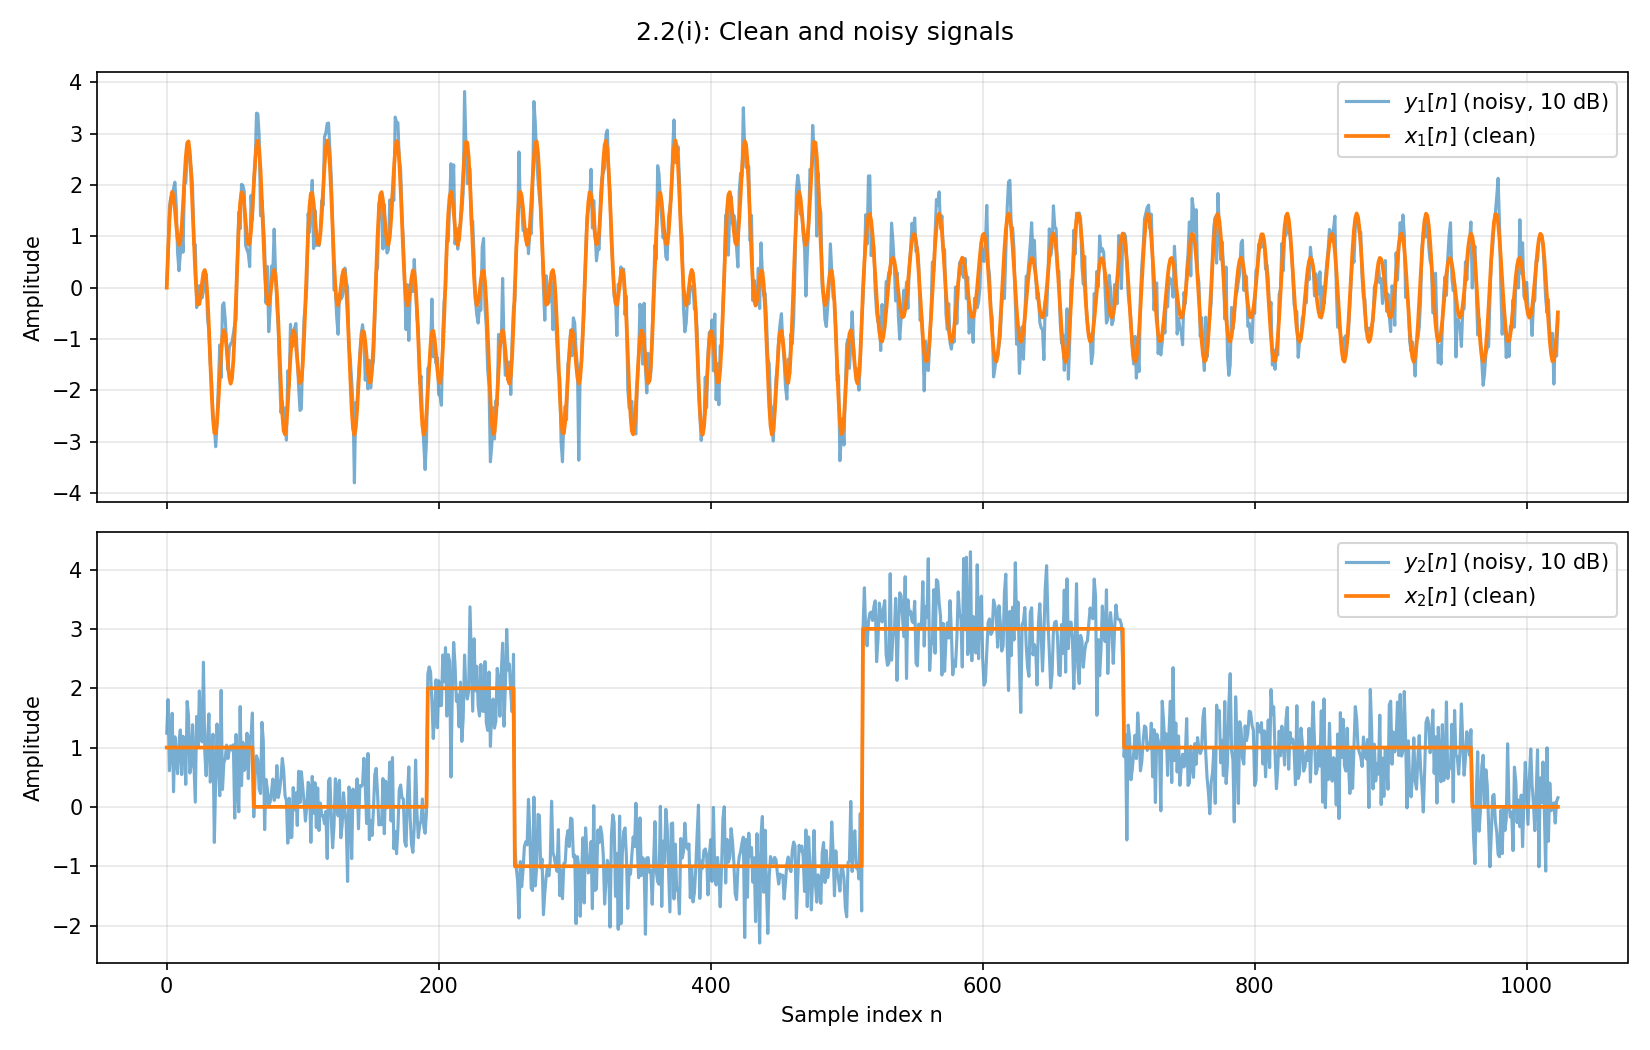
\includegraphics[width=0.9\textwidth]{fig2_2_i_signals.png}
    \caption{Clean signals $x_1[n]$, $x_2[n]$ and their noisy versions $y_1[n]$, $y_2[n]$ (10~dB SNR).}
    \label{fig:signals}
\end{figure}

\subsubsection*{(ii) Wavelet and scaling functions}

\begin{figure}[H]
    \centering
    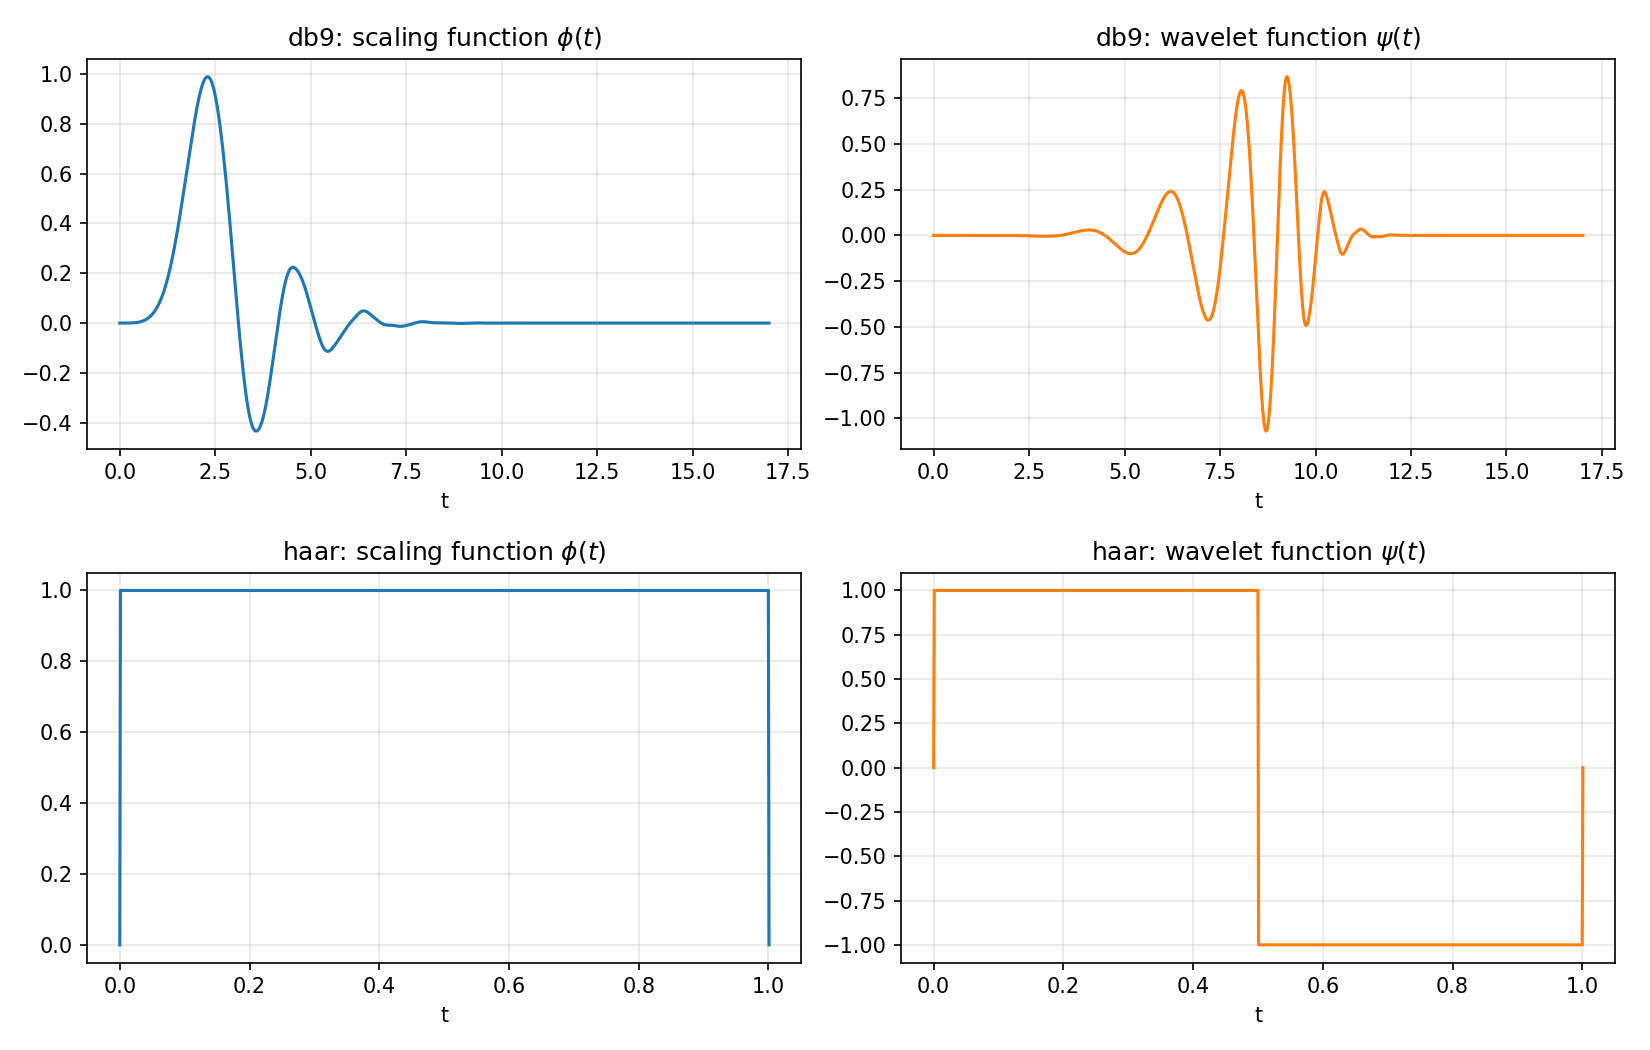
\includegraphics[width=0.85\textwidth]{fig2_2_ii_wavefun.png}
    \caption{Scaling function $\phi(t)$ and wavelet function $\psi(t)$ of Daubechies-9 and Haar, obtained with \texttt{wavefun()}.}
    \label{fig:wavefun}
\end{figure}

\begin{itemize}[leftmargin=*]
    \item \textbf{Haar:} the scaling function is a rectangular pulse on $[0,1)$ and the wavelet is a single positive/negative step. Both are discontinuous and have the shortest possible support (two filter taps) and only one vanishing moment. Haar is therefore very well localized in time but poorly localized in frequency.
    \item \textbf{db9:} the scaling and wavelet functions are smooth, oscillatory and asymmetric, with a support of length 17 (18 filter taps) and nine vanishing moments. The wavelet is better localized in frequency and can represent smooth, polynomial-like segments with very few coefficients, at the cost of a longer support in time.
\end{itemize}

\subsubsection*{(iii) 10-level decomposition}

The 10-level decomposition was computed with \texttt{pywt.wavedec(y, wavelet, level=10)} for both signals and both wavelets. The \texttt{periodization} boundary mode was used so that the transform is non-redundant and orthogonal: the 1024 samples give exactly 1024 coefficients, arranged as
\[
    [\,cA_{10}, cD_{10}, cD_9, \dots, cD_1\,] \quad\text{with lengths}\quad [1, 1, 2, 4, 8, 16, 32, 64, 128, 256, 512].
\]
At each level the approximation is low-pass and high-pass filtered and down-sampled by two, so $cD_j$ covers the band $[f_s/2^{j+1},\, f_s/2^{j}]$; for example $cD_1$ covers 128--256~Hz and $cD_5$ covers 8--16~Hz. (For db9, ten levels exceed the maximum level at which the filter is shorter than the signal, so PyWavelets issues a boundary-effect warning; the decomposition nevertheless remains perfectly invertible.)

The coefficients are shown in Figures~\ref{fig:coeffs_y1} and~\ref{fig:coeffs_y2}.

\begin{figure}[H]
    \centering
    \begin{subfigure}{0.49\textwidth}
        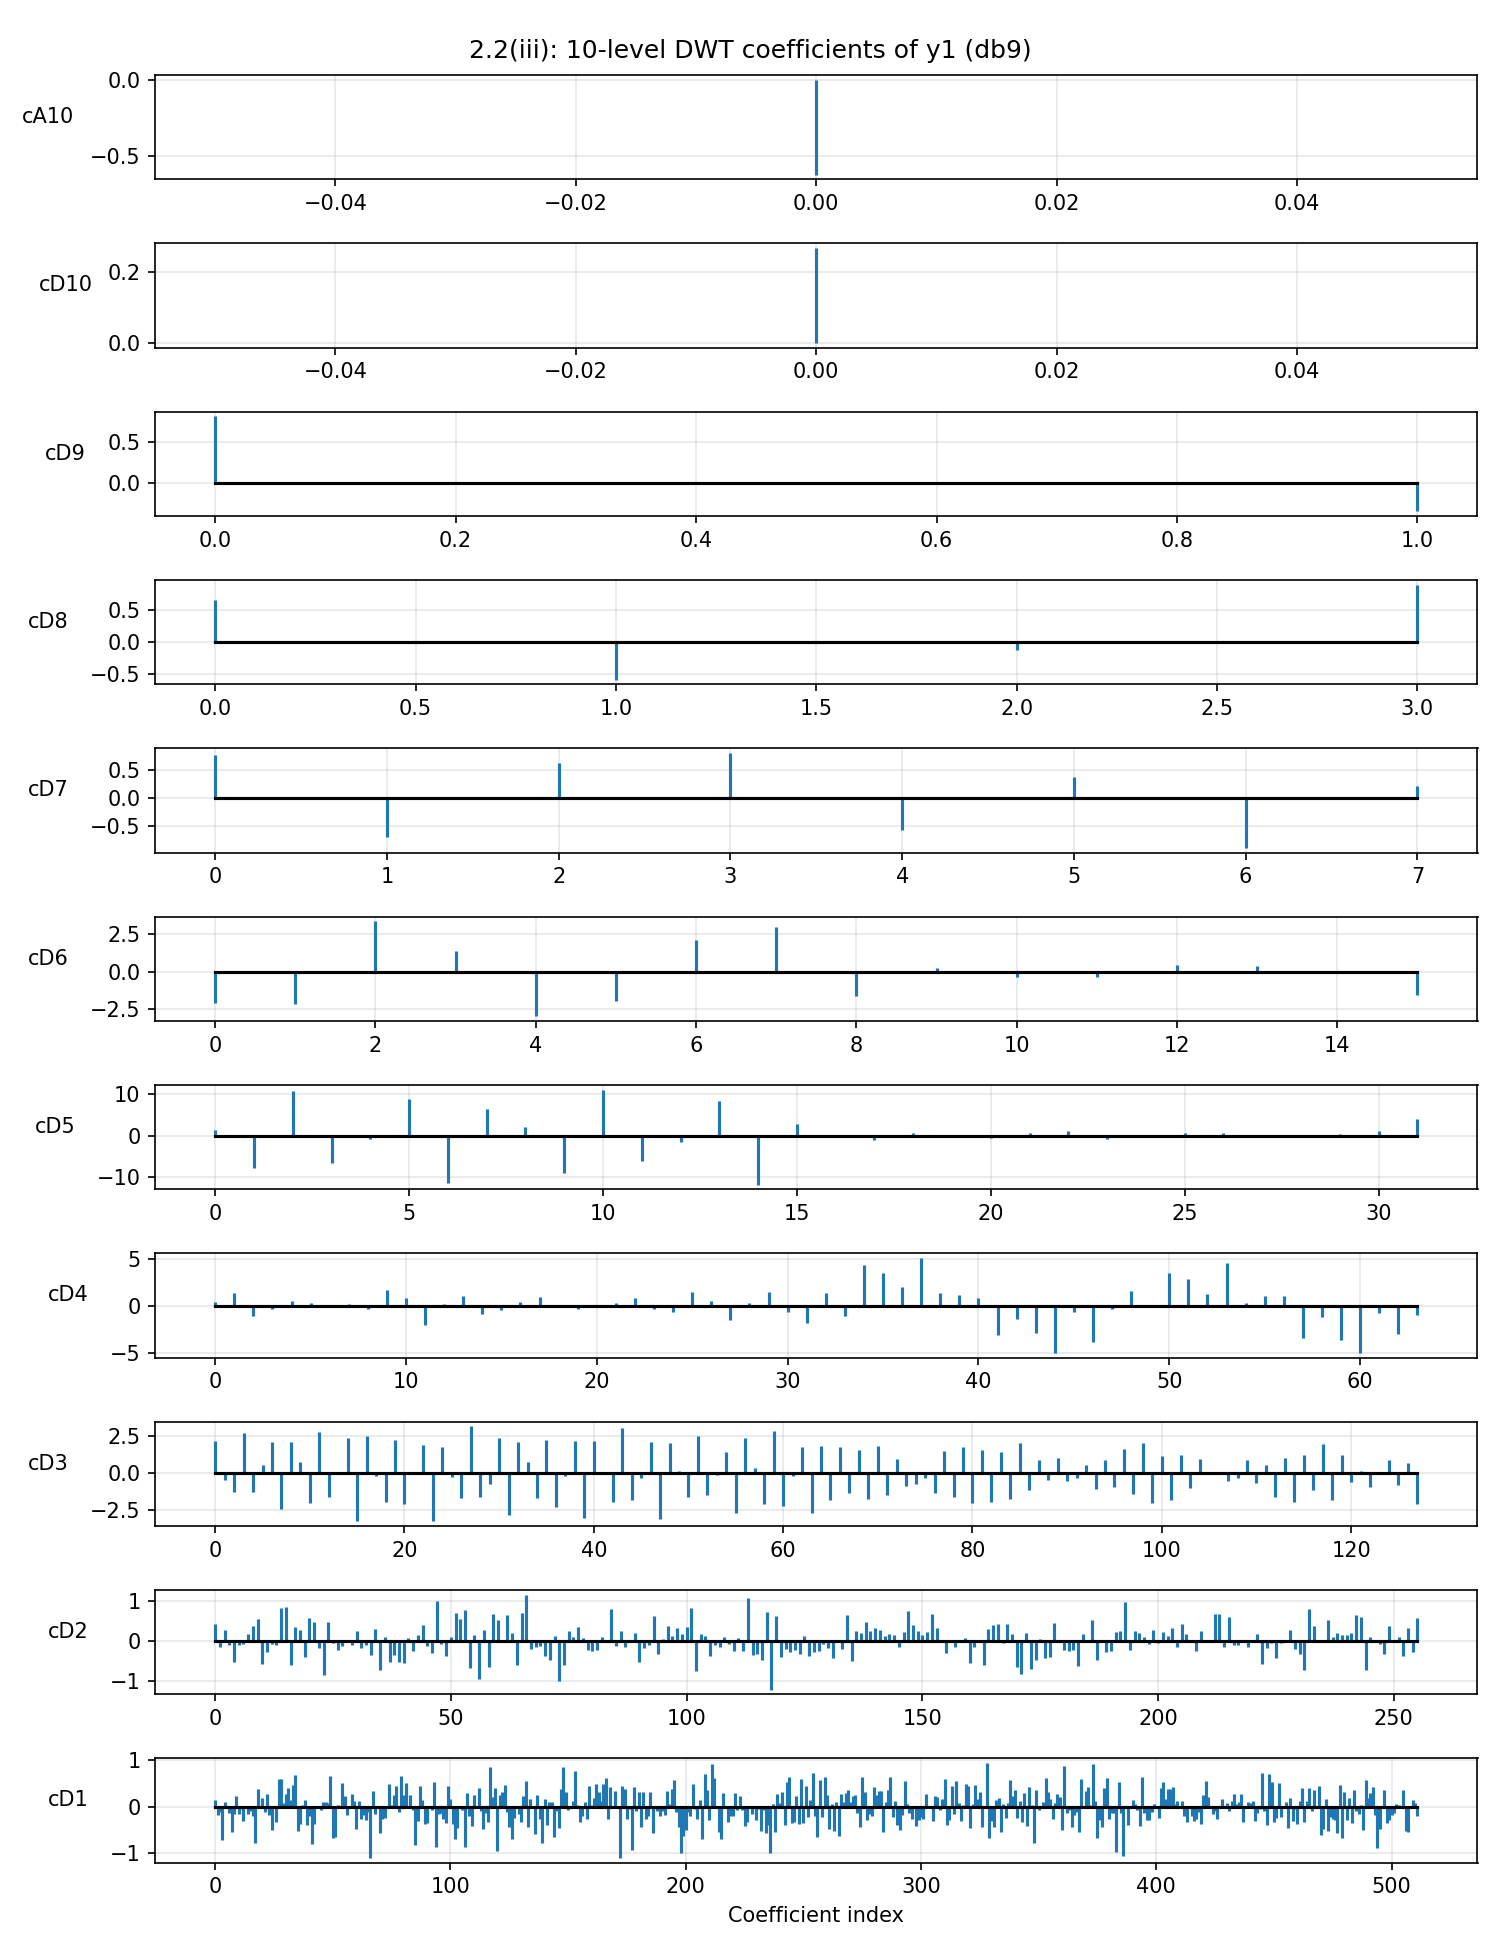
\includegraphics[width=\textwidth]{fig2_2_iii_coeffs_y1_db9.png}
        \caption{db9}
    \end{subfigure}
    \begin{subfigure}{0.49\textwidth}
        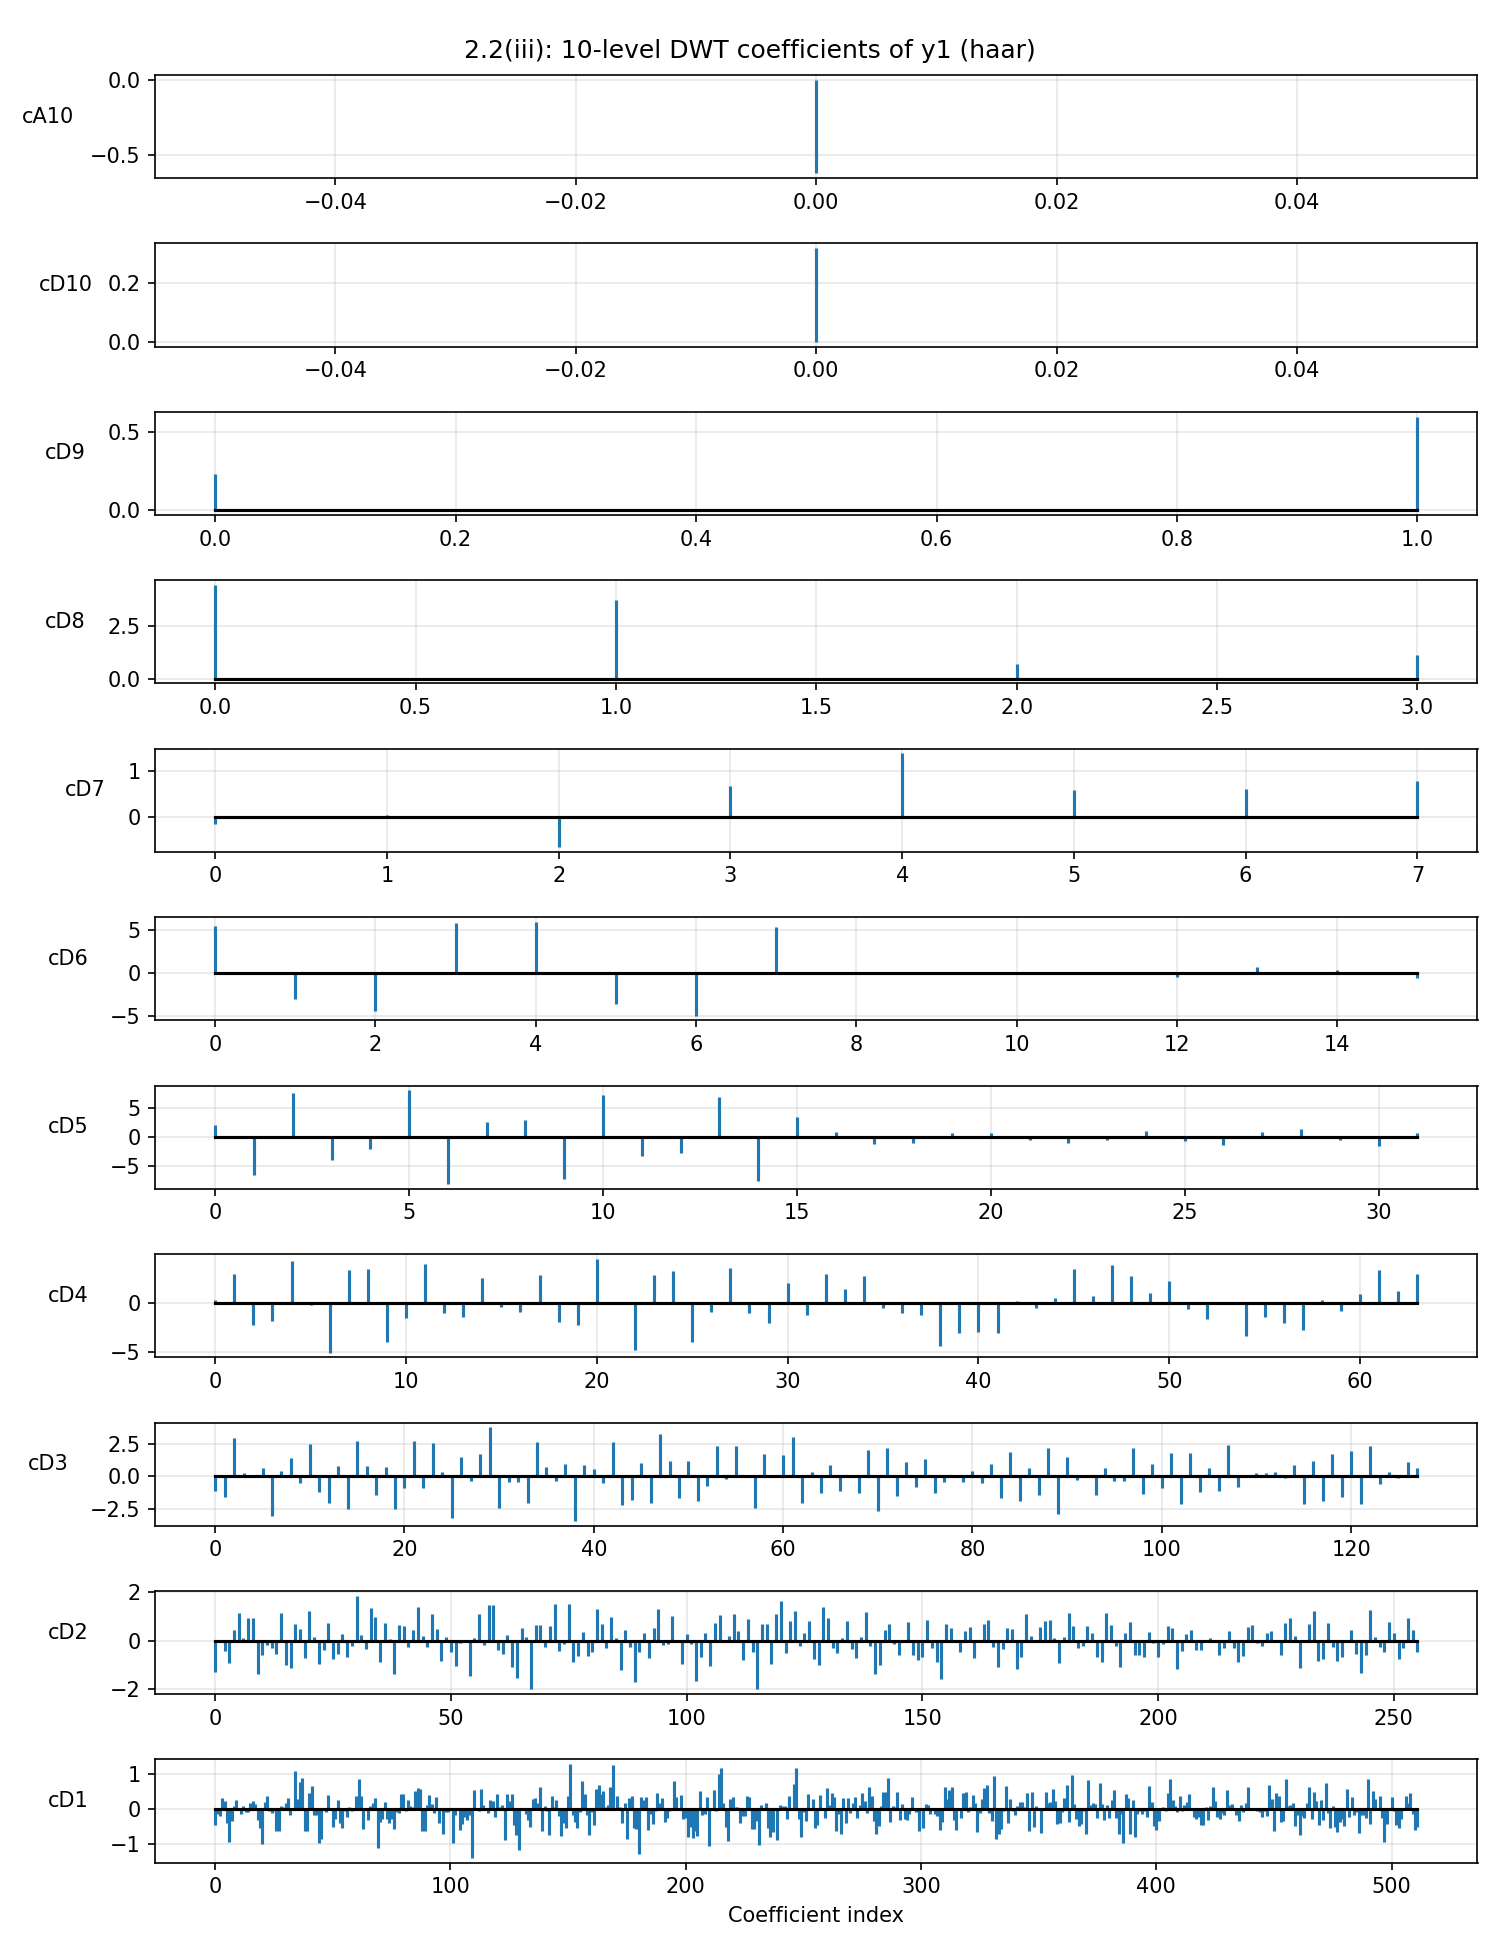
\includegraphics[width=\textwidth]{fig2_2_iii_coeffs_y1_haar.png}
        \caption{Haar}
    \end{subfigure}
    \caption{10-level DWT coefficients $cA_{10}, cD_{10}, \dots, cD_1$ of $y_1$.}
    \label{fig:coeffs_y1}
\end{figure}

\begin{figure}[H]
    \centering
    \begin{subfigure}{0.49\textwidth}
        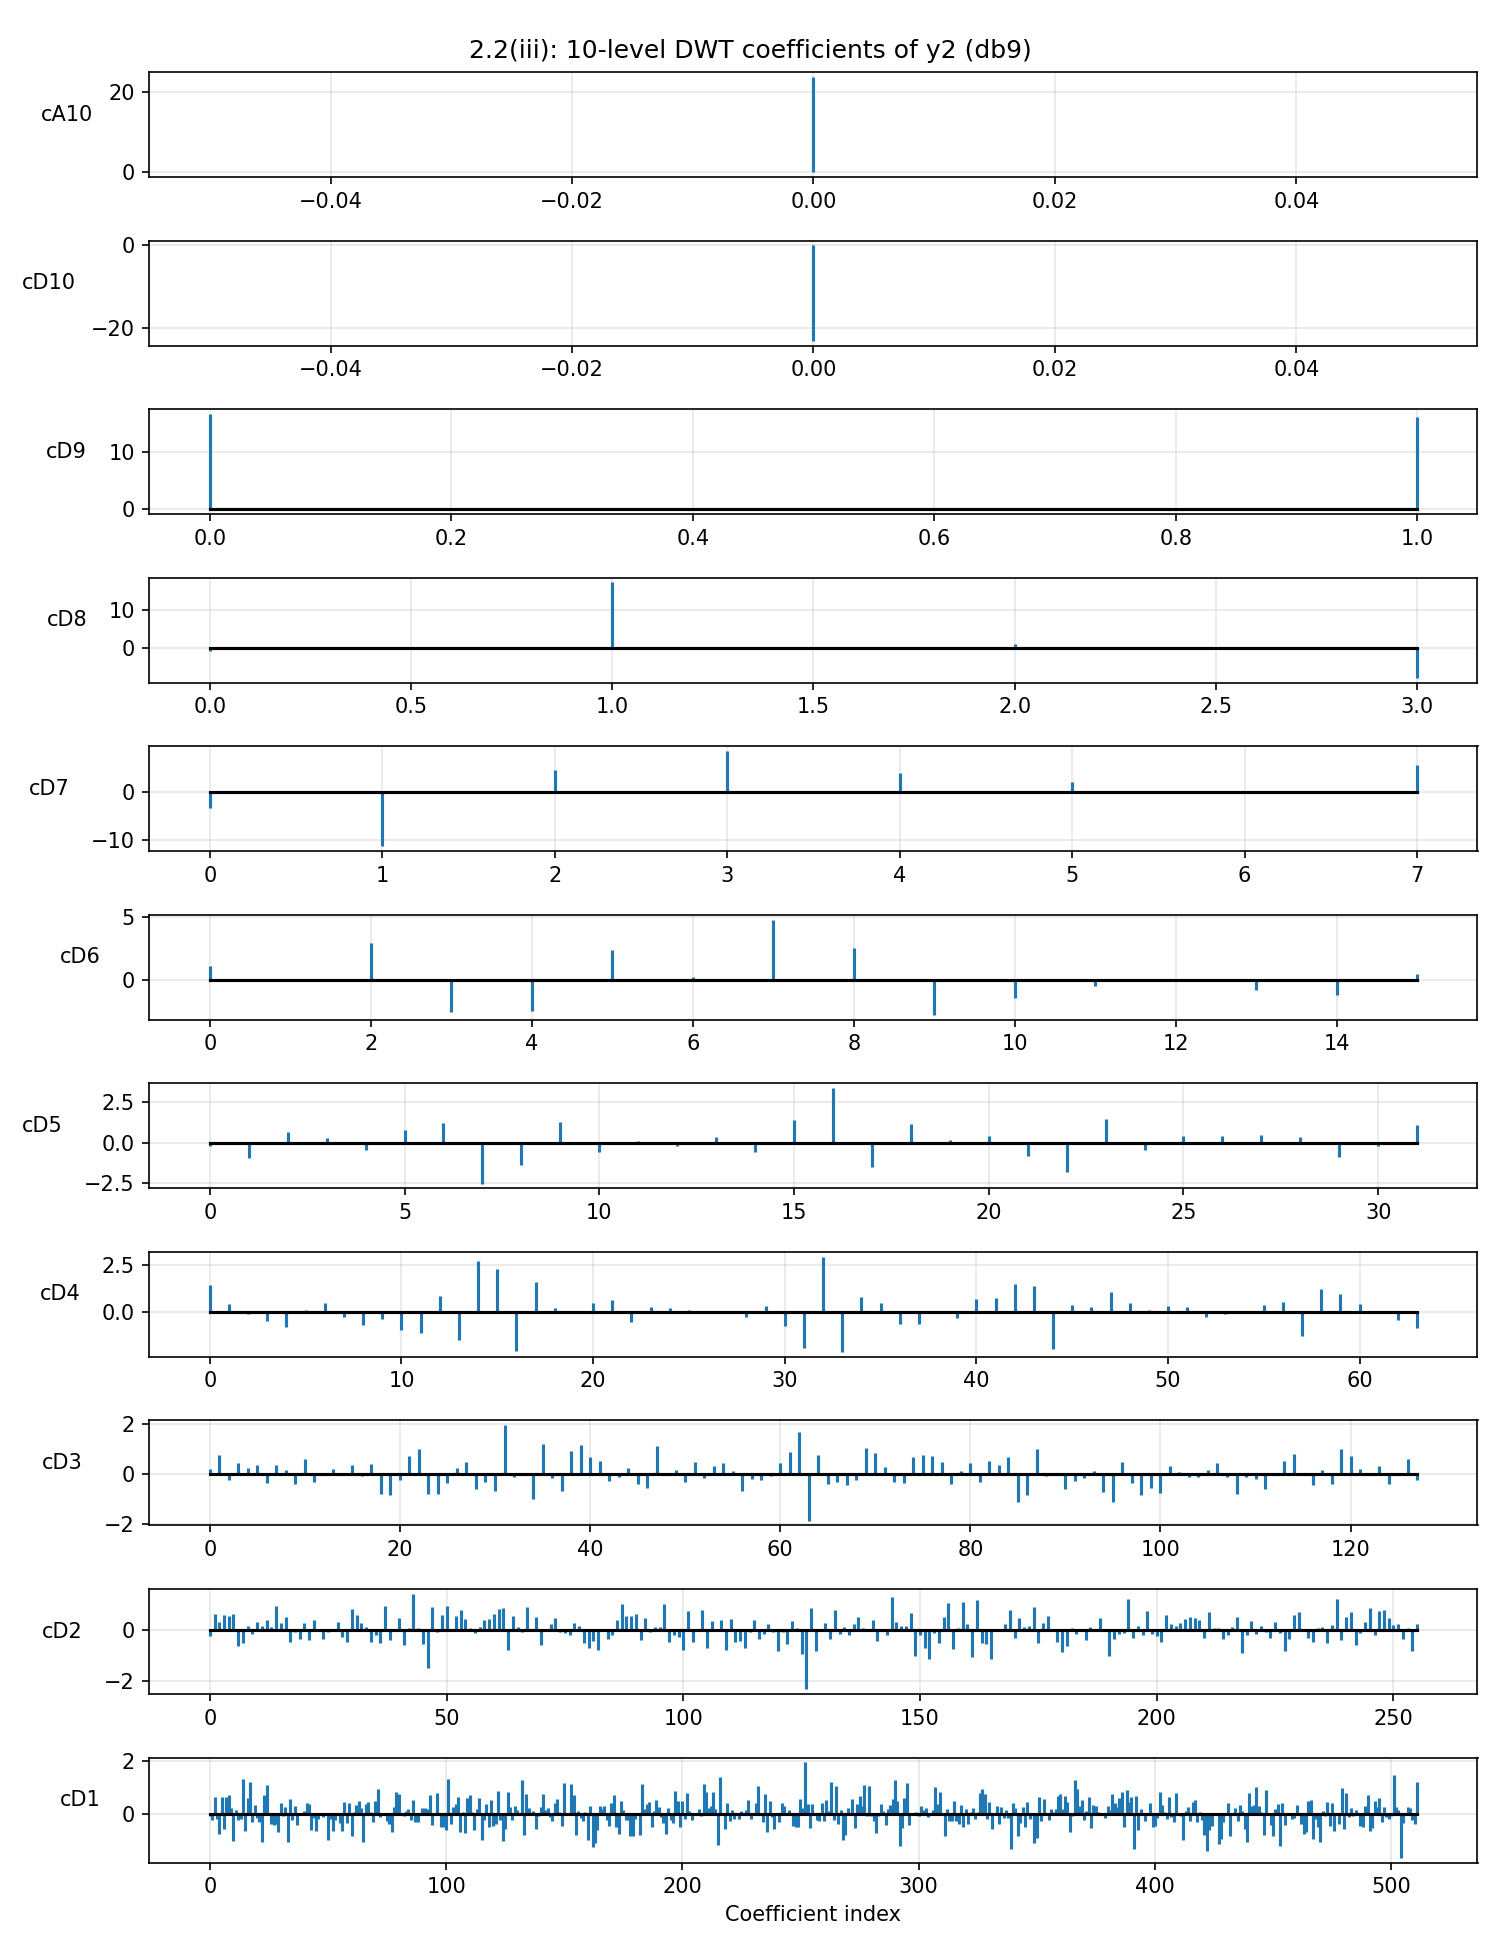
\includegraphics[width=\textwidth]{fig2_2_iii_coeffs_y2_db9.png}
        \caption{db9}
    \end{subfigure}
    \begin{subfigure}{0.49\textwidth}
        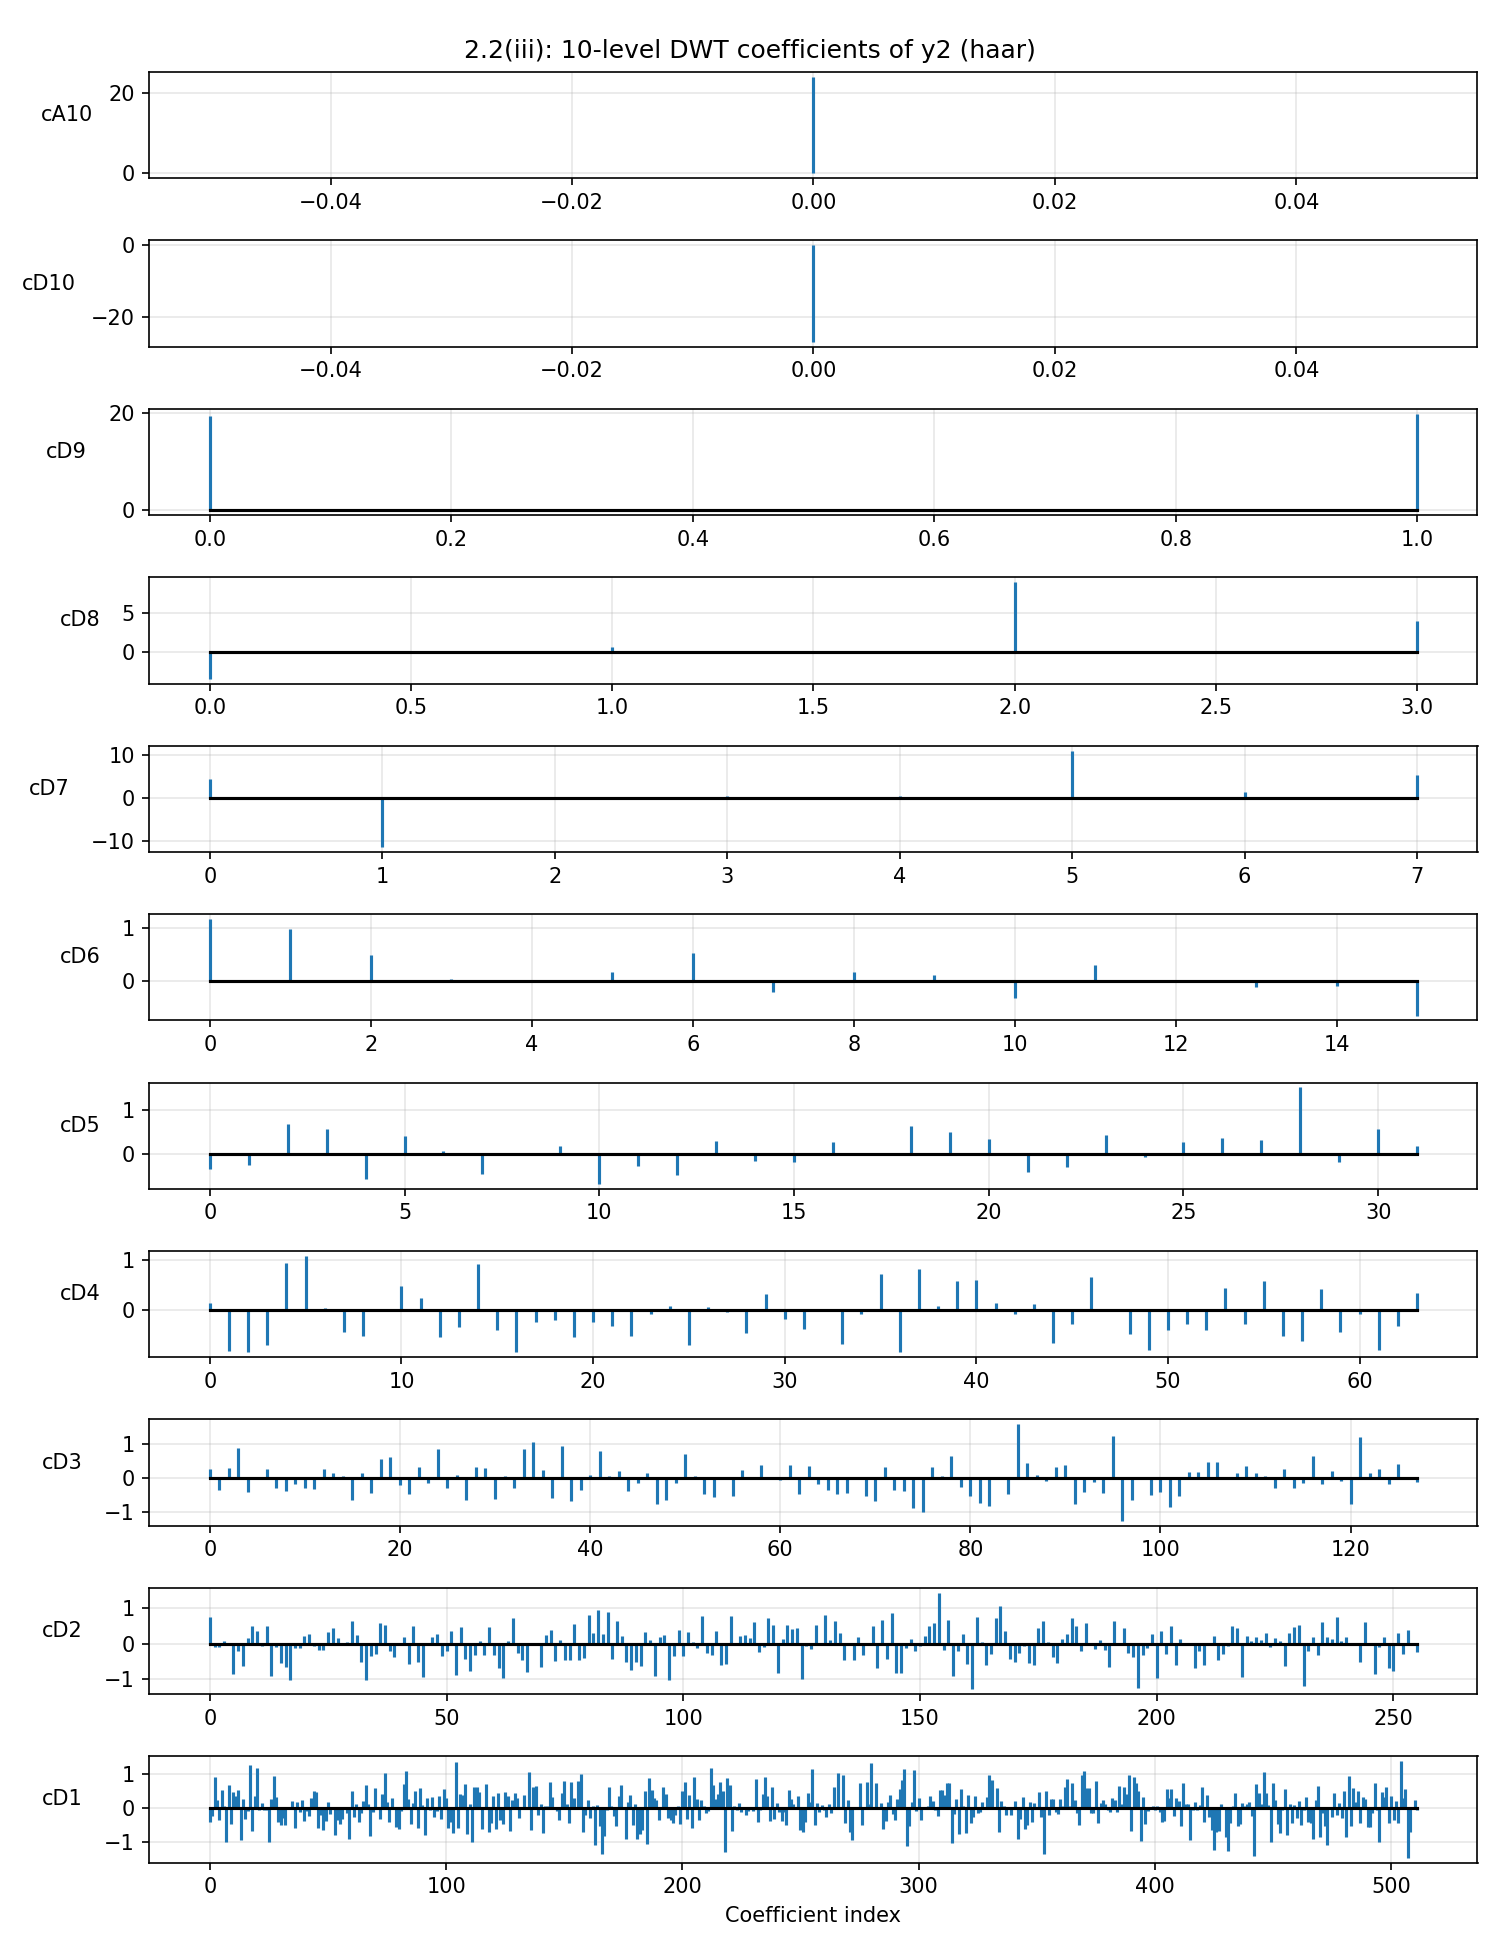
\includegraphics[width=\textwidth]{fig2_2_iii_coeffs_y2_haar.png}
        \caption{Haar}
    \end{subfigure}
    \caption{10-level DWT coefficients $cA_{10}, cD_{10}, \dots, cD_1$ of $y_2$.}
    \label{fig:coeffs_y2}
\end{figure}

The number of coefficients halves at each level, so the fine-scale detail bands ($cD_1$, $cD_2$) contain most of the coefficients and the coarsest bands contain only one or two. In the fine-scale bands the coefficients are small and noise-like for both signals, whereas the signal energy is carried by a limited number of large coefficients in the middle and coarse bands. This sparsity is what the denoising and compression in the following sections rely on.

\subsubsection*{(iv) Reconstruction of $A_{10}, D_{10}, \dots, D_1$}

The steps followed were:
\begin{enumerate}[leftmargin=*]
    \item Decompose $y$ into the coefficient list $[cA_{10}, cD_{10}, \dots, cD_1]$.
    \item To reconstruct one sub-band, keep the corresponding coefficient array and replace all the other arrays with zeros, then apply the inverse DWT (\texttt{pywt.waverec}). This gives the contribution of that sub-band alone at the full signal length. Repeating this for every array gives $A_{10}, D_{10}, \dots, D_1$.
    \item Add the components, $\hat{y} = A_{10} + \sum_{i=1}^{10} D_i$. Because the inverse DWT is linear, this sum must equal the inverse transform of the complete coefficient set, i.e.\ the original signal.
    \item Compare the energy of $y$ and $\hat{y}$ and compute the energy of the difference, $\sum_n (y[n] - \hat{y}[n])^2$.
\end{enumerate}

\begin{table}[H]
    \centering
    \begin{tabular}{llccc}
        \toprule
        Signal & Wavelet & $E(y)$ & $E(\hat{y})$ & $E(y - \hat{y})$ \\
        \midrule
        $y_1$ & db9  & 1755.721985 & 1755.721985 & $2.39\times10^{-28}$ \\
        $y_1$ & Haar & 1755.721985 & 1755.721985 & $7.48\times10^{-28}$ \\
        $y_2$ & db9  & 2745.187532 & 2745.187532 & $9.71\times10^{-28}$ \\
        $y_2$ & Haar & 2745.187532 & 2745.187532 & $3.64\times10^{-27}$ \\
        \bottomrule
    \end{tabular}
    \caption{Energy of the noisy signal, of the sum of the reconstructed sub-bands and of their difference.}
    \label{tab:energy}
\end{table}

The energies are identical and the energy of the difference is of the order of $10^{-27}$, i.e.\ floating-point round-off. Hence $y = A_{10} + \sum_{i=1}^{10} D_i$ is verified for both signals and both wavelets (perfect reconstruction). The reconstructed sub-bands are shown in Figures~\ref{fig:comp_y1} and~\ref{fig:comp_y2}.

\begin{figure}[H]
    \centering
    \begin{subfigure}{0.49\textwidth}
        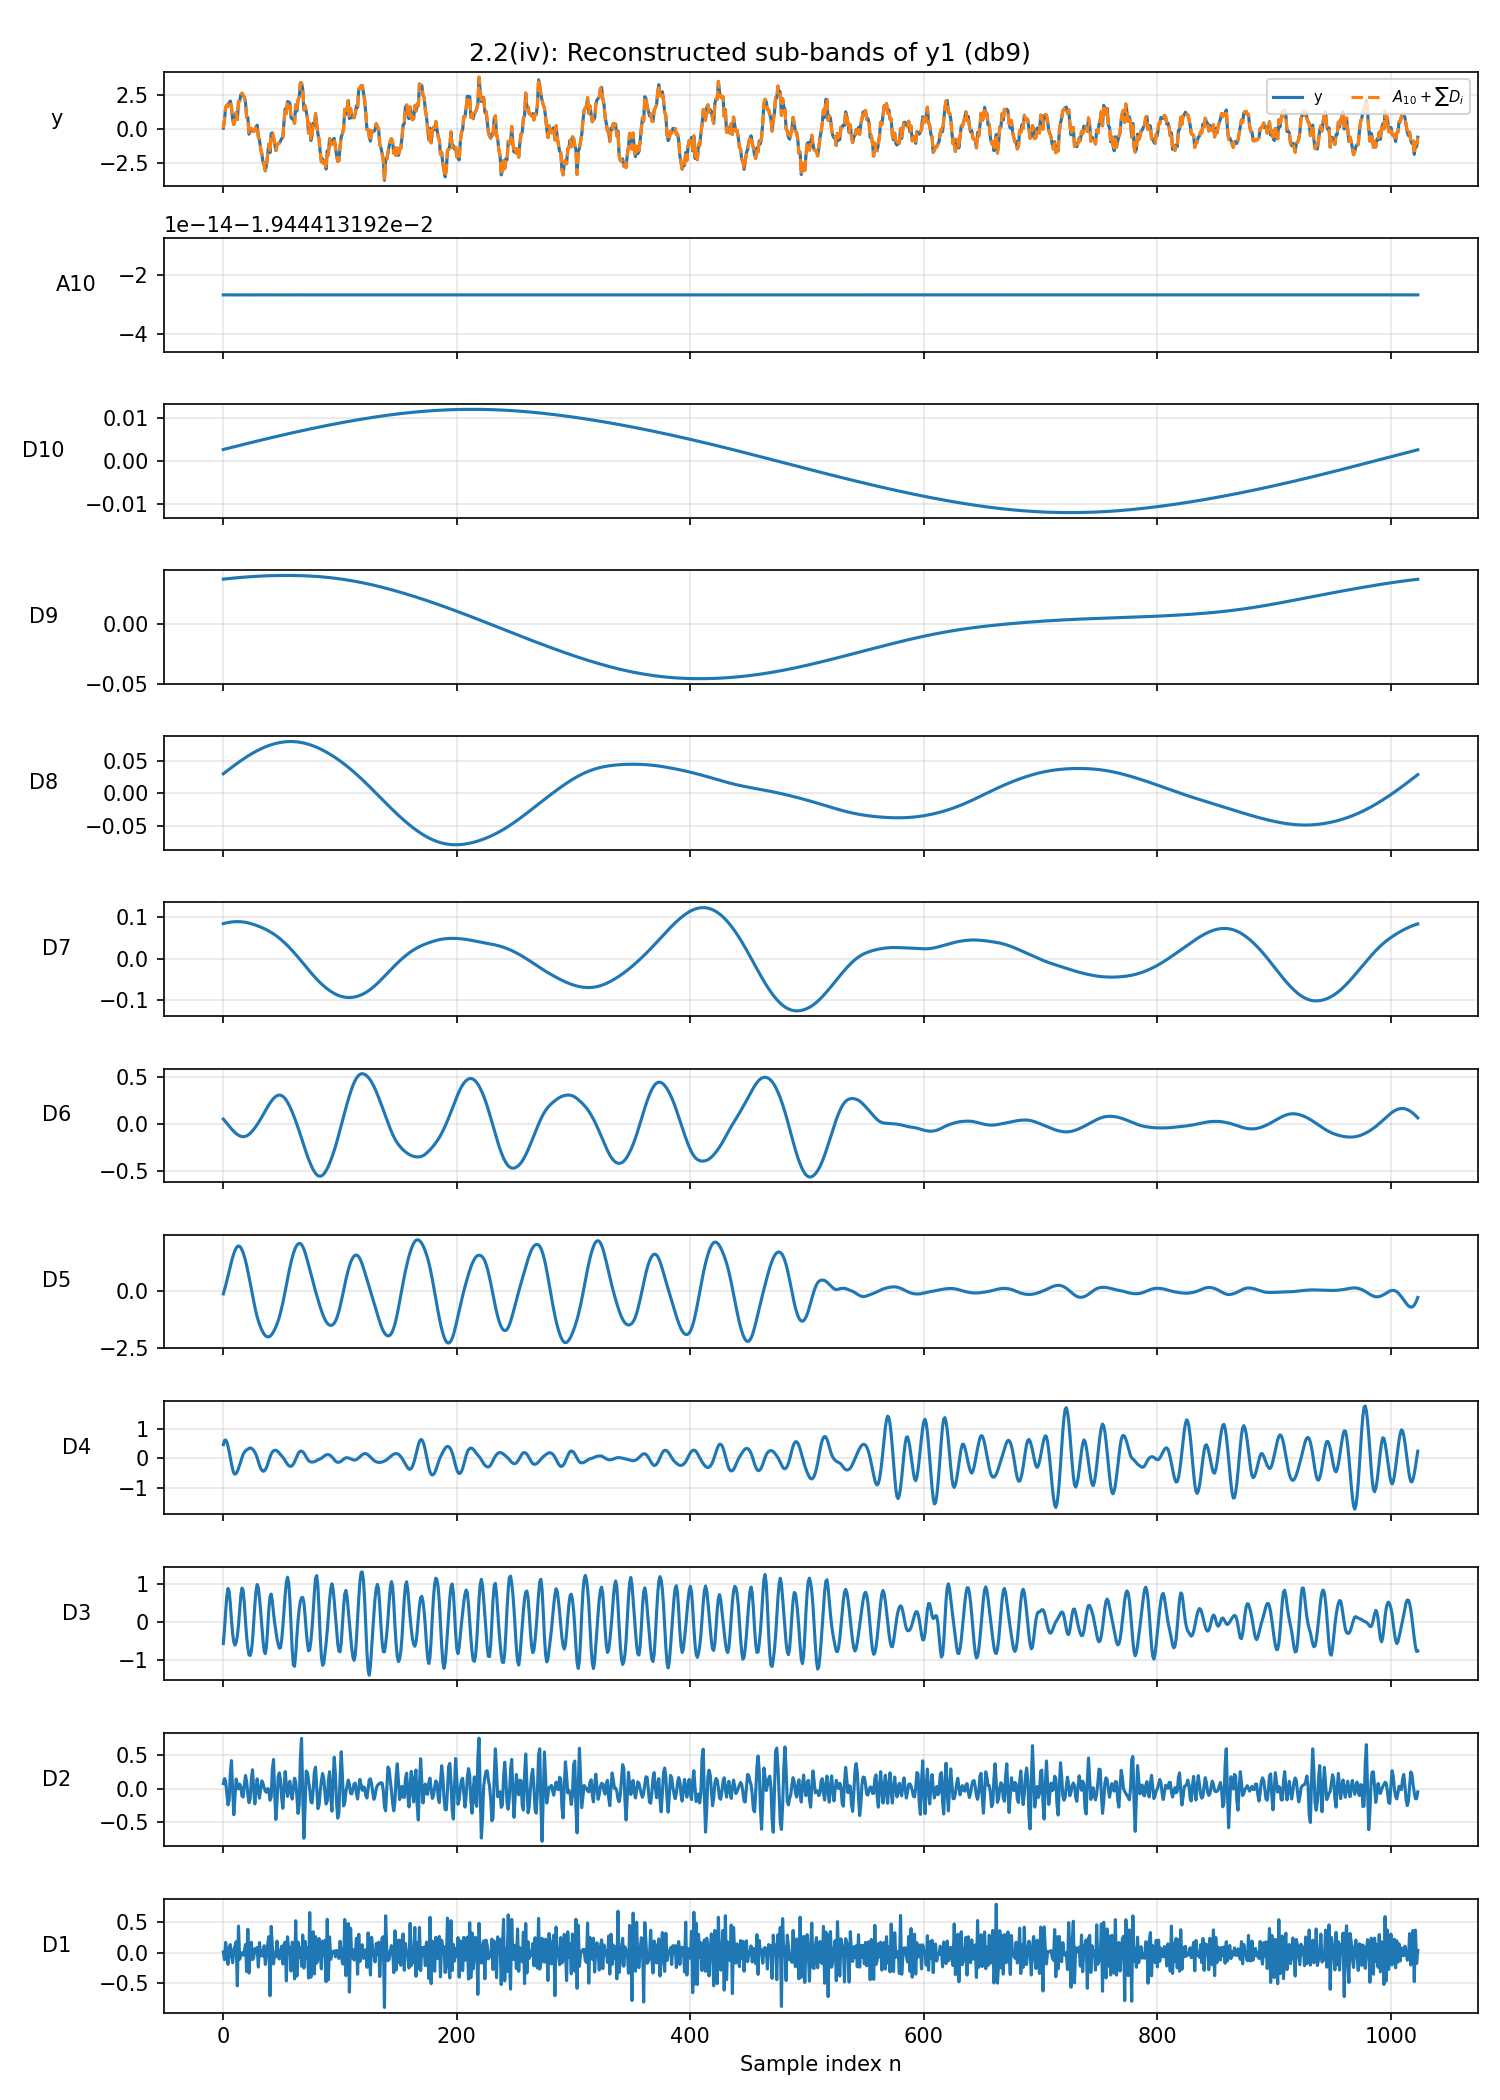
\includegraphics[width=\textwidth]{fig2_2_iv_components_y1_db9.png}
        \caption{db9}
    \end{subfigure}
    \begin{subfigure}{0.49\textwidth}
        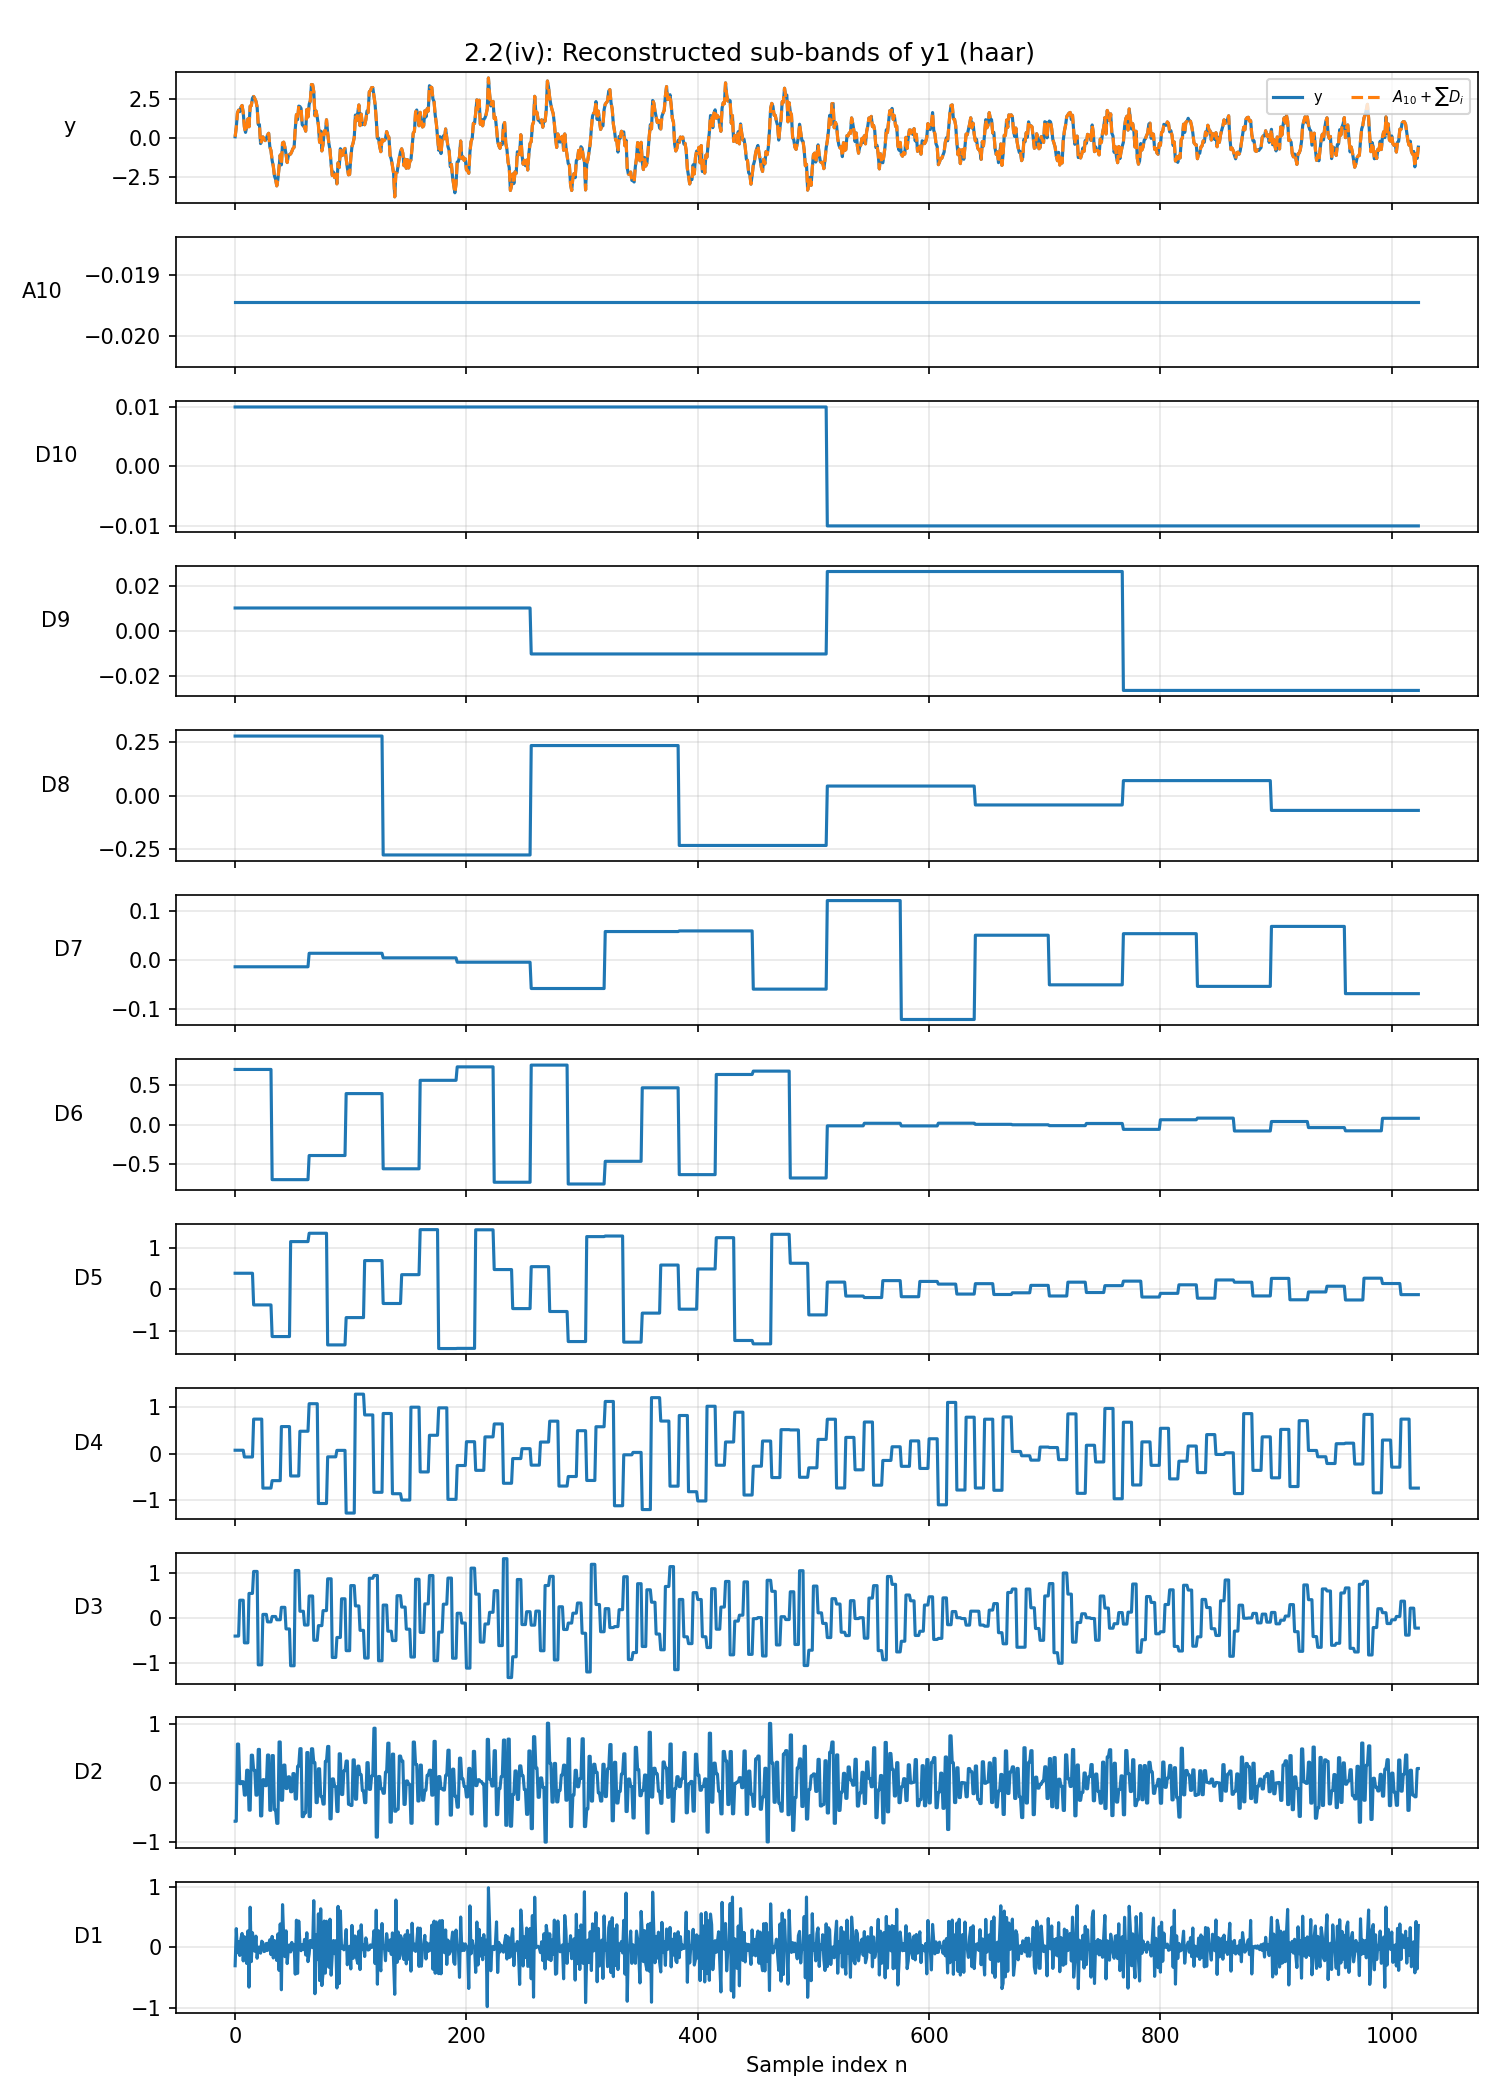
\includegraphics[width=\textwidth]{fig2_2_iv_components_y1_haar.png}
        \caption{Haar}
    \end{subfigure}
    \caption{Reconstructed sub-bands $A_{10}, D_{10}, \dots, D_1$ of $y_1$.}
    \label{fig:comp_y1}
\end{figure}

\begin{figure}[H]
    \centering
    \begin{subfigure}{0.49\textwidth}
        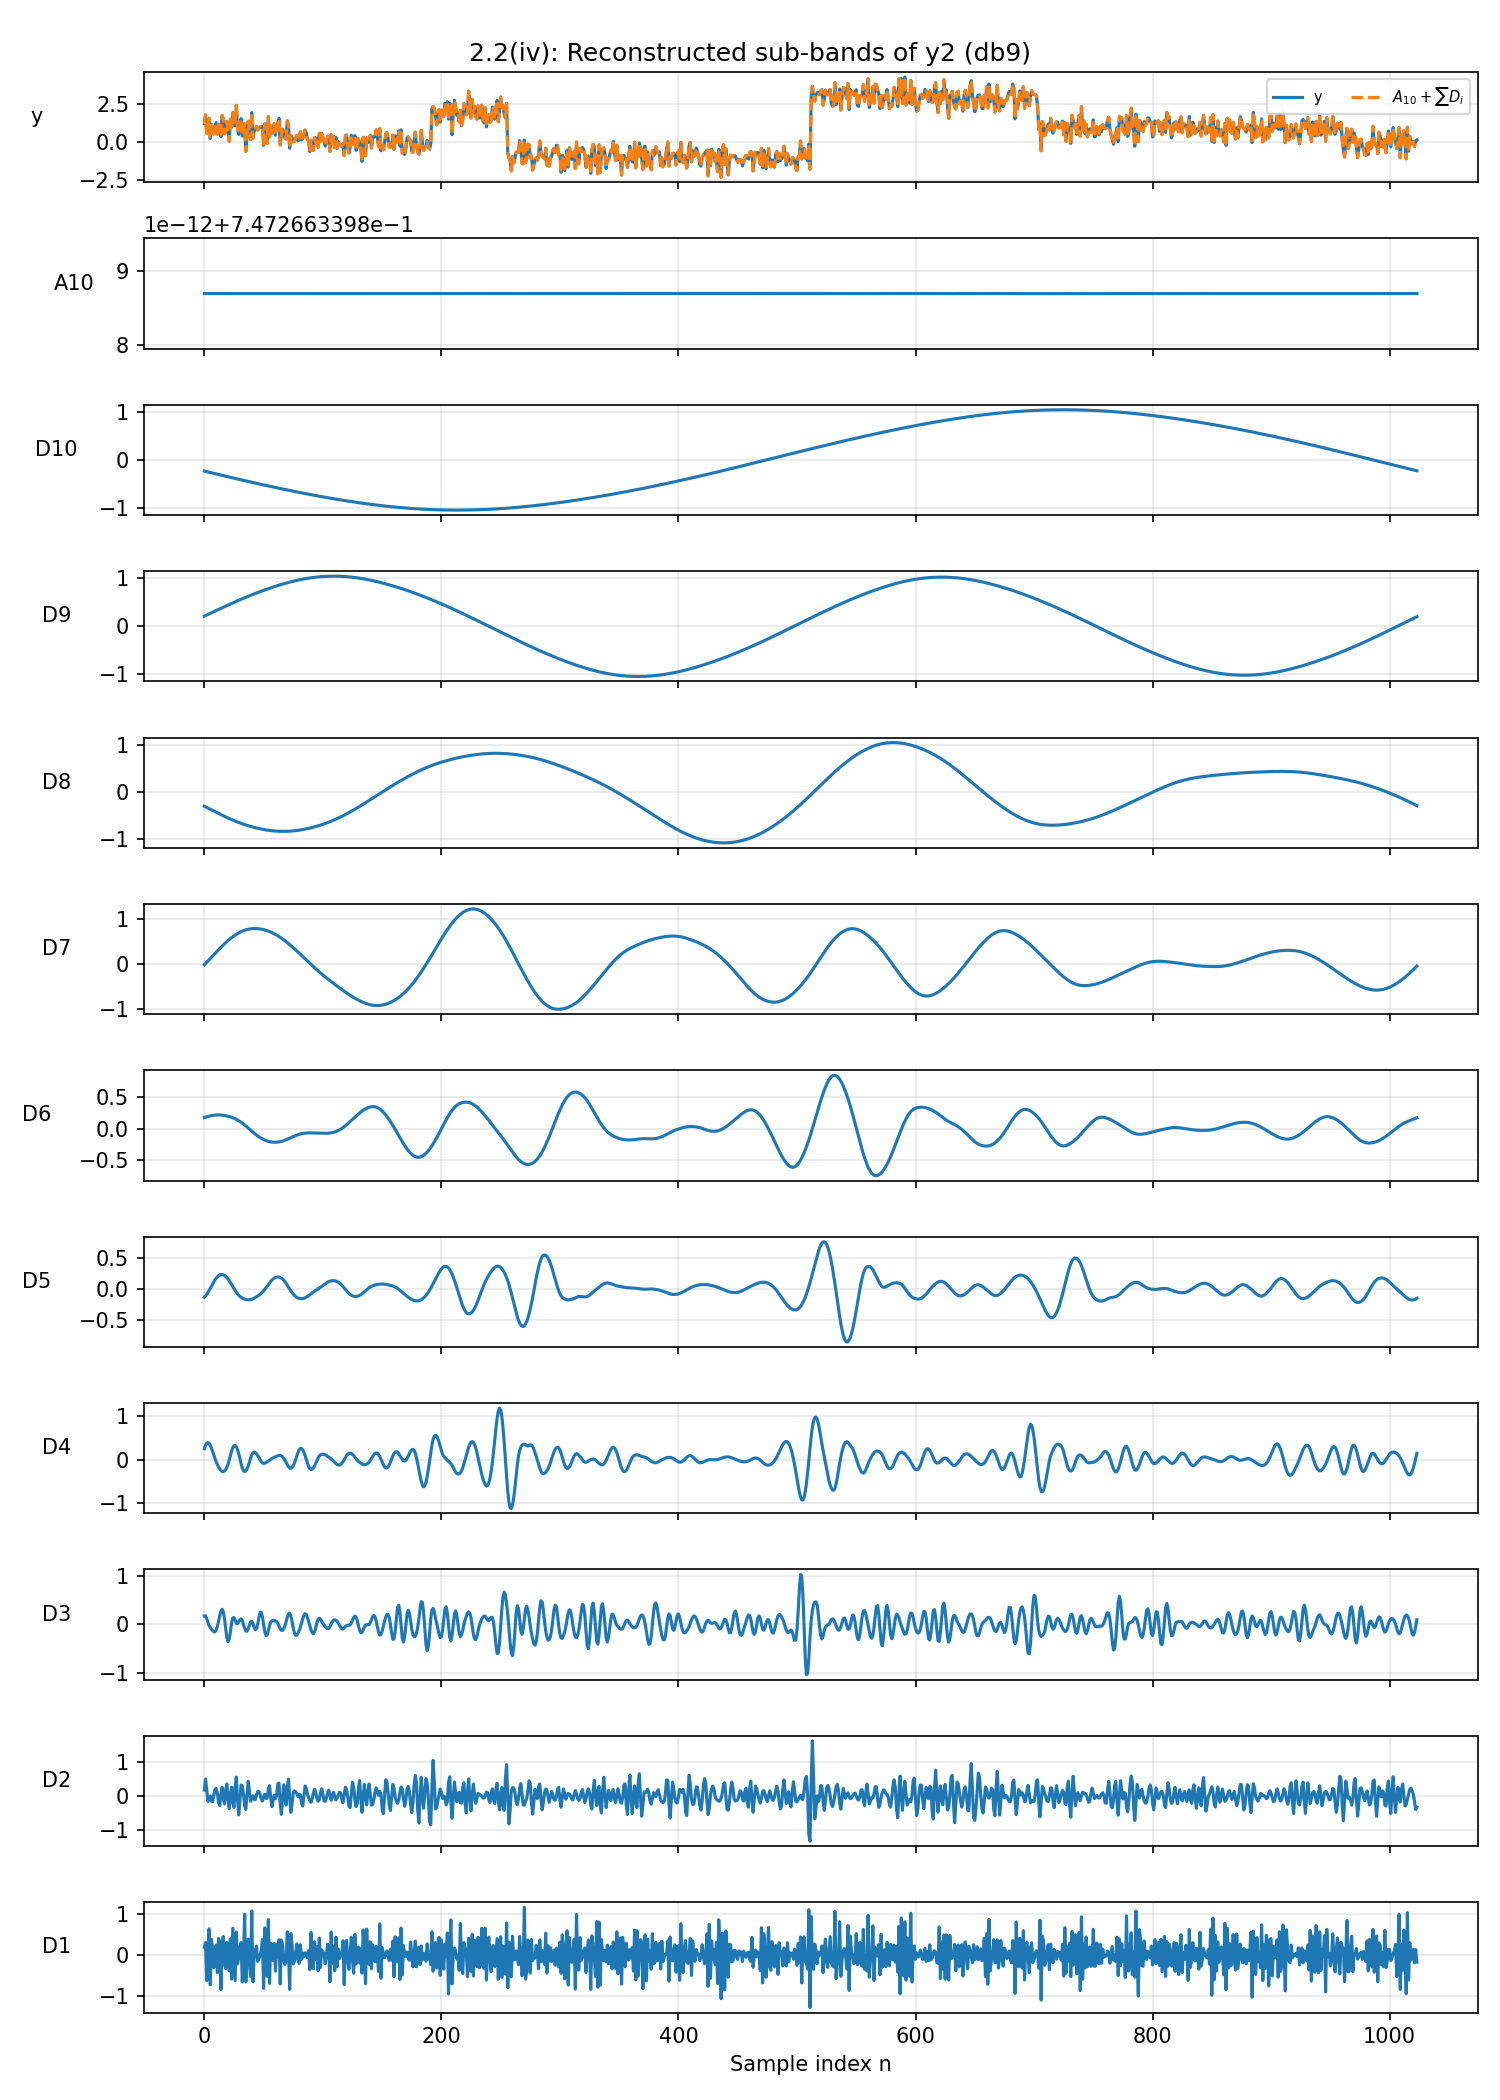
\includegraphics[width=\textwidth]{fig2_2_iv_components_y2_db9.png}
        \caption{db9}
    \end{subfigure}
    \begin{subfigure}{0.49\textwidth}
        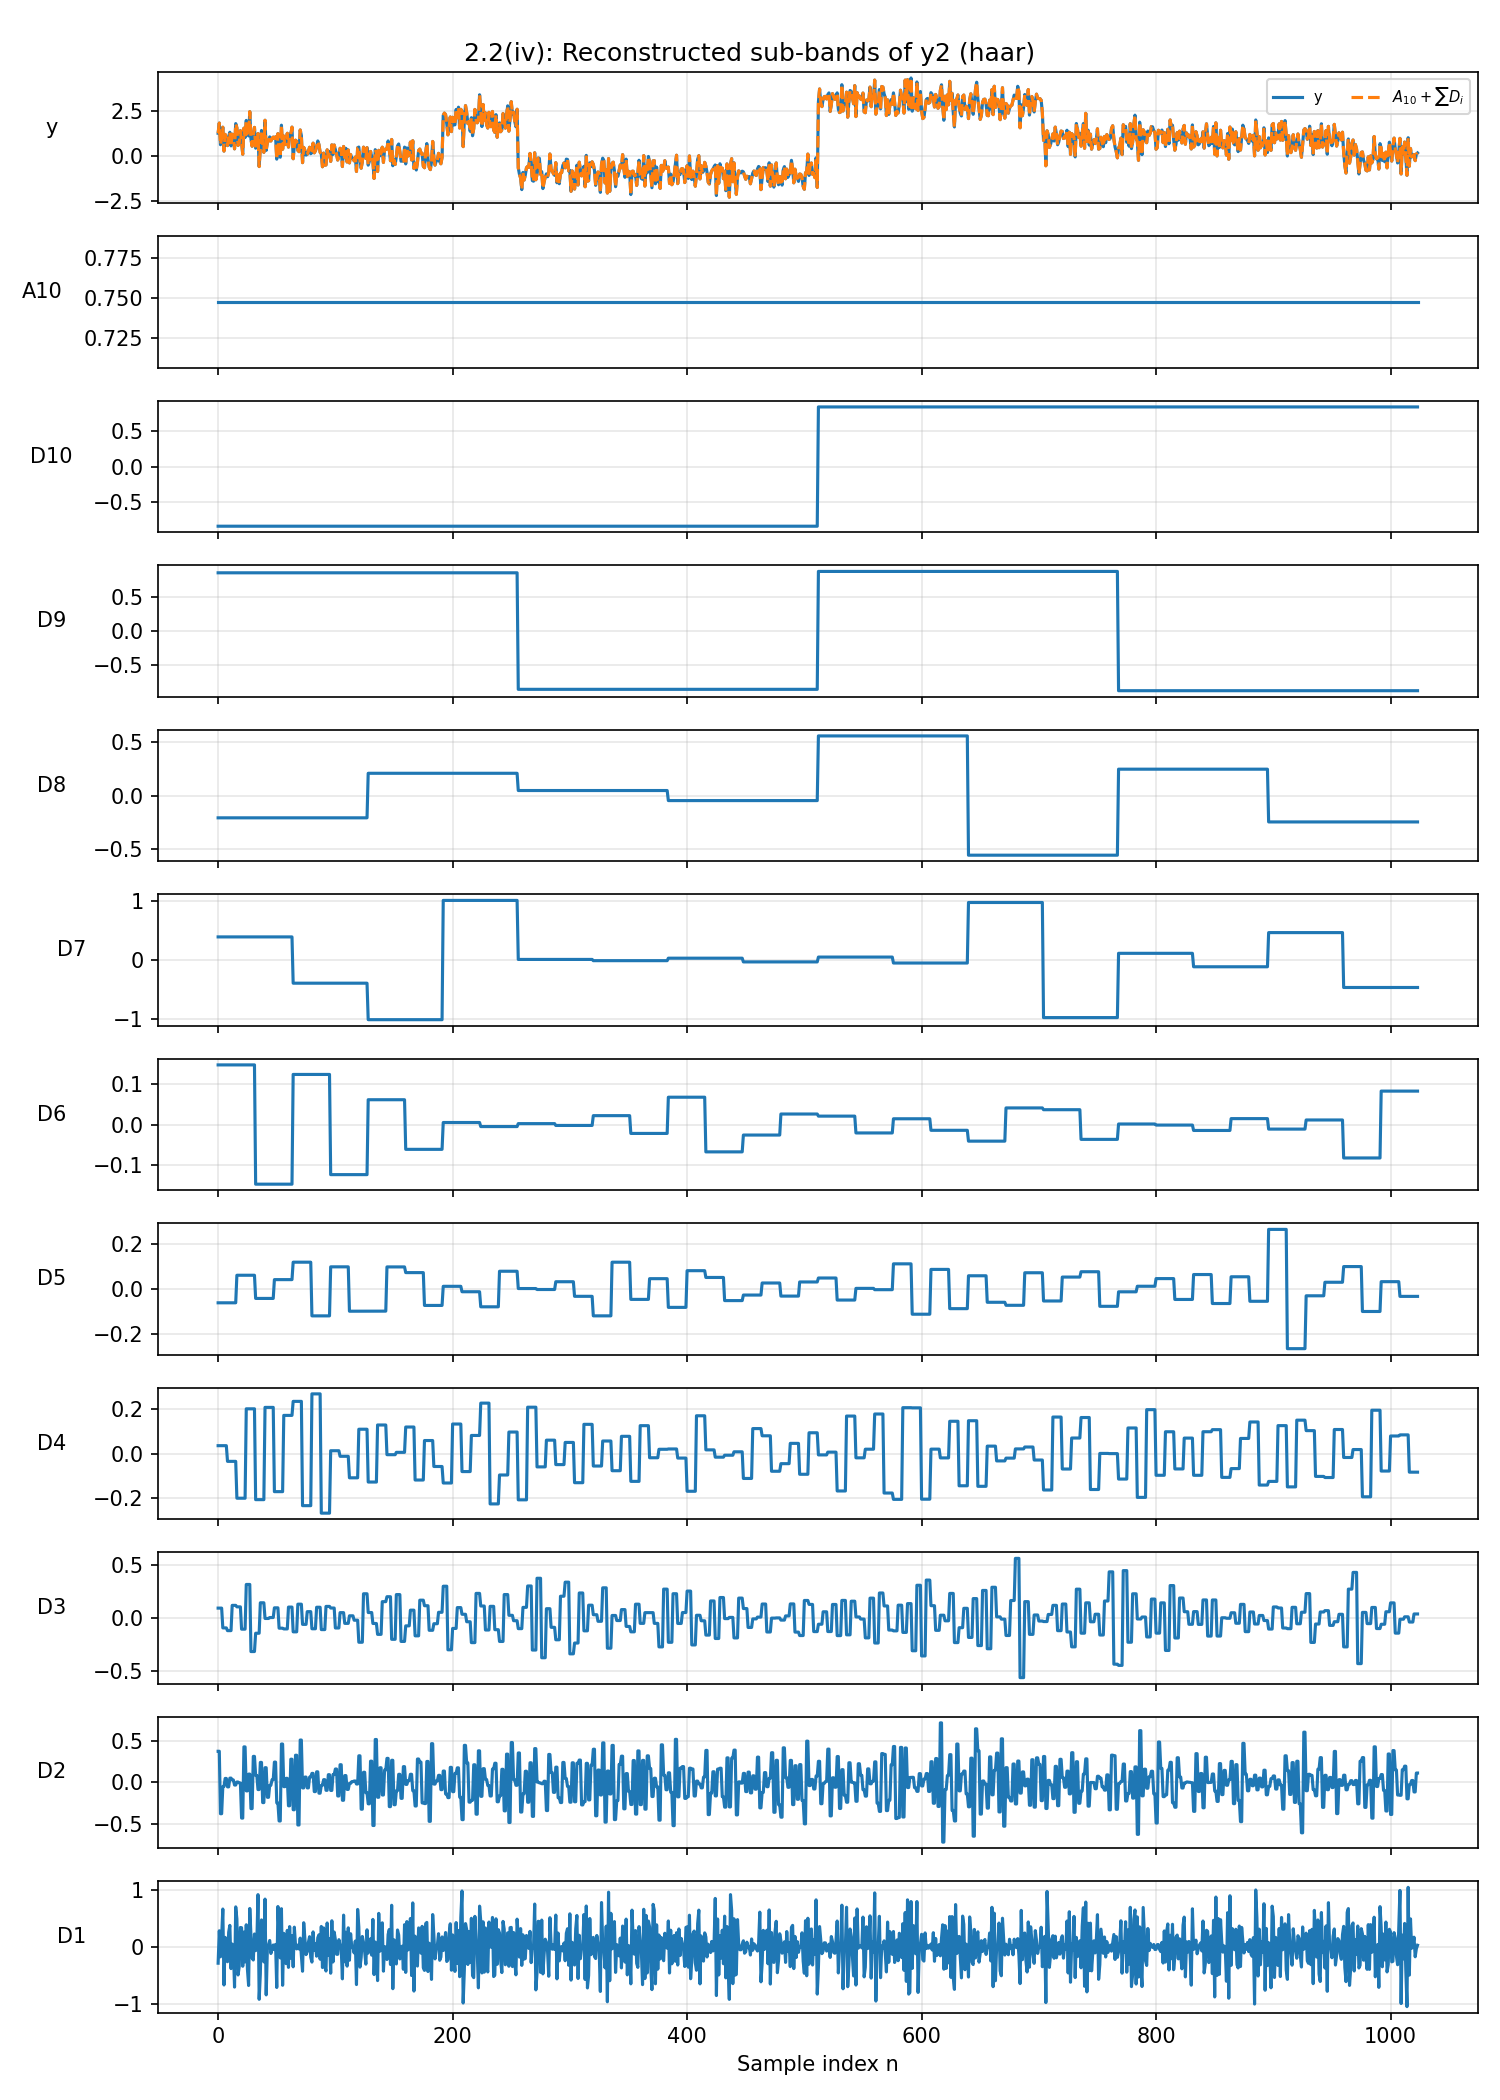
\includegraphics[width=\textwidth]{fig2_2_iv_components_y2_haar.png}
        \caption{Haar}
    \end{subfigure}
    \caption{Reconstructed sub-bands $A_{10}, D_{10}, \dots, D_1$ of $y_2$.}
    \label{fig:comp_y2}
\end{figure}

For $y_1$ with db9 the sub-bands separate the sinusoids cleanly: the 10~Hz component appears in $D_5$ (8--16~Hz) and the 40~Hz component in $D_3$ (32--64~Hz) during the first half, while the 20~Hz and 30~Hz components appear mainly in $D_4$ (16--32~Hz) during the second half. $D_1$ and $D_2$ contain almost only noise. The DWT therefore shows both which frequency bands are active and when they are active.

\subsection{Signal denoising with the DWT}

\subsubsection*{(i) Sorted coefficient magnitudes}

All the coefficients of each decomposition were concatenated and their magnitudes sorted in descending order (Figure~\ref{fig:sorted}).

\begin{figure}[H]
    \centering
    \begin{subfigure}{0.49\textwidth}
        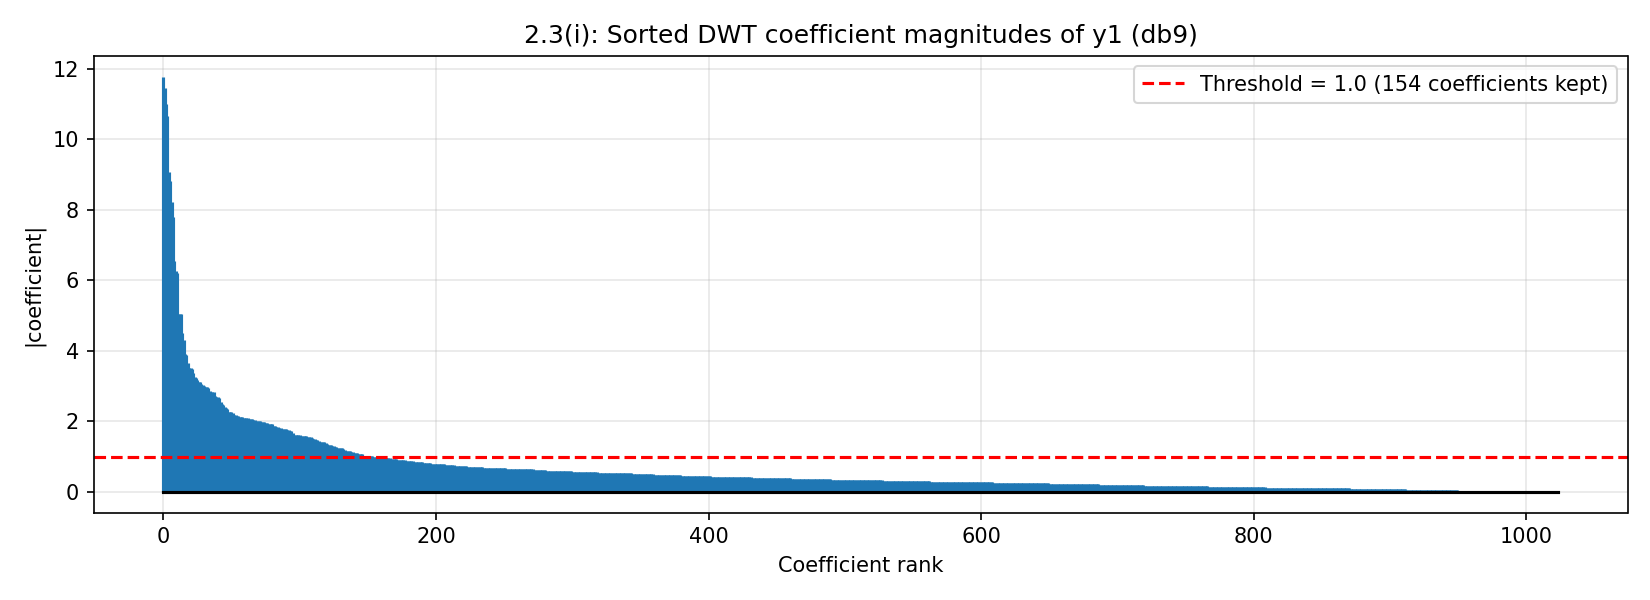
\includegraphics[width=\textwidth]{fig2_3_i_sorted_coeffs_y1_db9.png}
        \caption{$y_1$, db9}
    \end{subfigure}
    \begin{subfigure}{0.49\textwidth}
        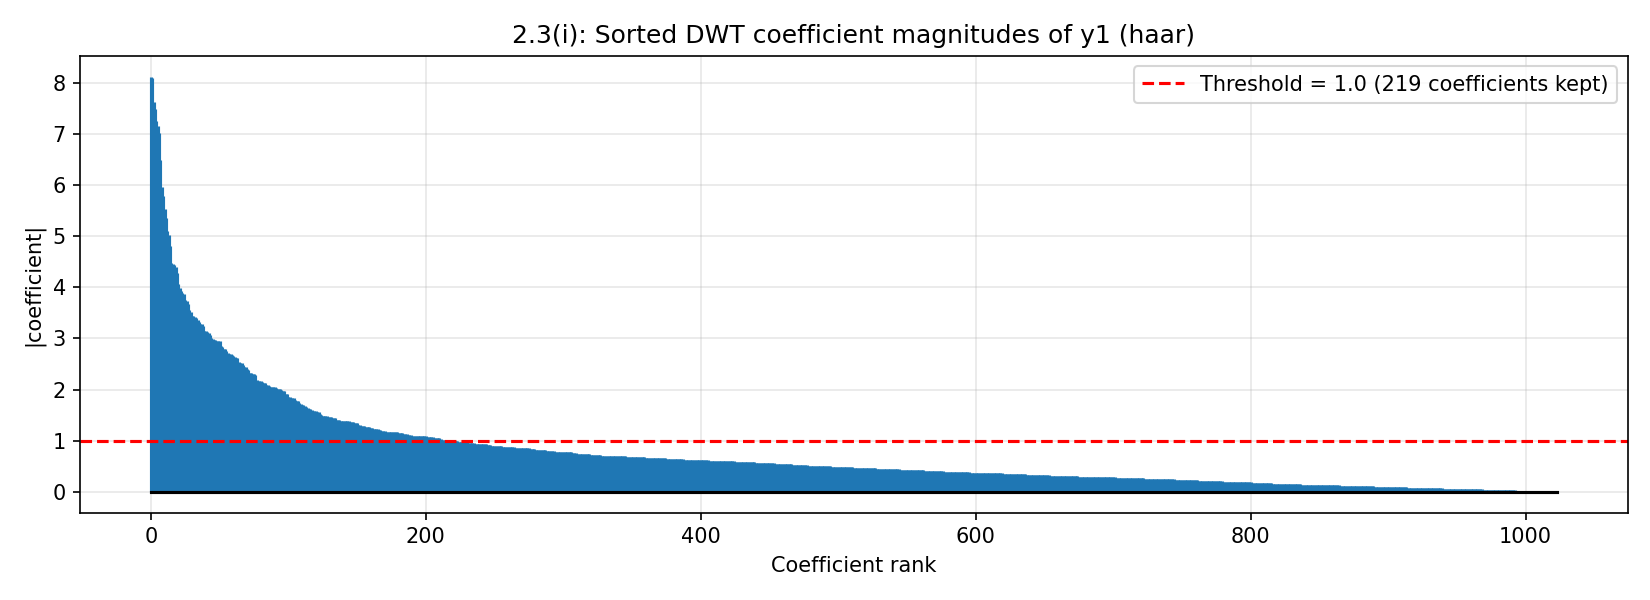
\includegraphics[width=\textwidth]{fig2_3_i_sorted_coeffs_y1_haar.png}
        \caption{$y_1$, Haar}
    \end{subfigure}
    \begin{subfigure}{0.49\textwidth}
        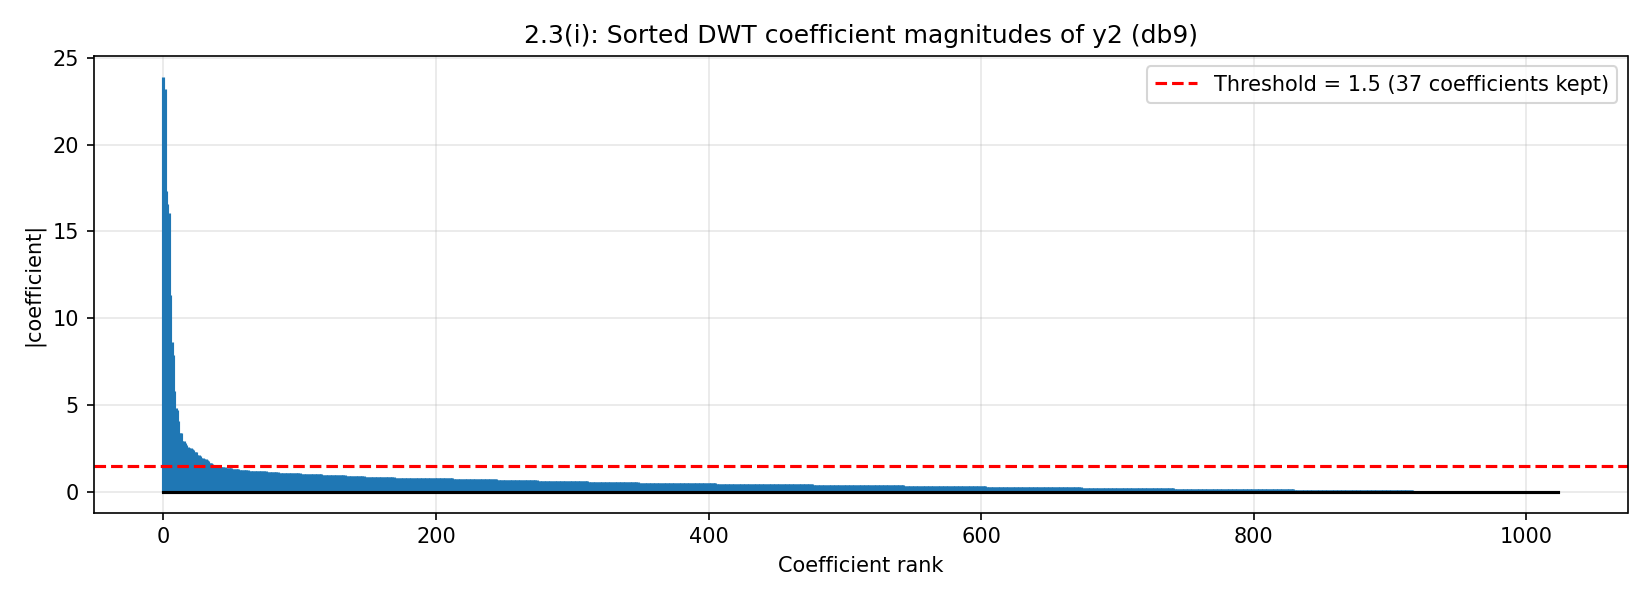
\includegraphics[width=\textwidth]{fig2_3_i_sorted_coeffs_y2_db9.png}
        \caption{$y_2$, db9}
    \end{subfigure}
    \begin{subfigure}{0.49\textwidth}
        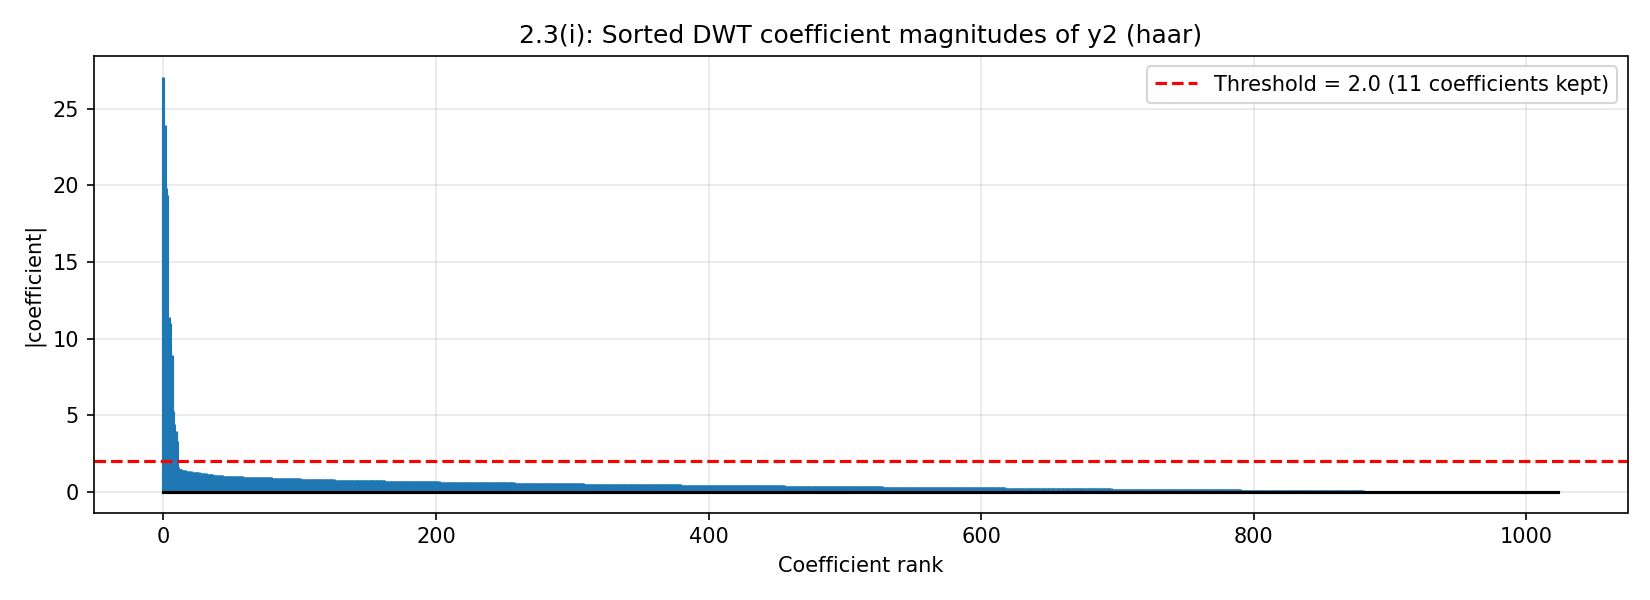
\includegraphics[width=\textwidth]{fig2_3_i_sorted_coeffs_y2_haar.png}
        \caption{$y_2$, Haar}
    \end{subfigure}
    \caption{DWT coefficient magnitudes in descending order with the selected thresholds.}
    \label{fig:sorted}
\end{figure}

In every case a small number of large coefficients is followed by a long, slowly decaying tail. Because the transform is orthogonal, white noise is spread evenly over all coefficients with the same variance, whereas the signal is concentrated in a few large coefficients. The tail therefore mostly represents noise.

\subsubsection*{(ii) Threshold selection and reconstruction}

The threshold was chosen by observation at the knee of each curve, where the steep part meets the flat noise floor: 1.0 for $y_1$ with both wavelets, 1.5 for $y_2$ with db9 and 2.0 for $y_2$ with Haar. Coefficients with a magnitude below the threshold were set to zero (hard thresholding) and the signal was reconstructed with the inverse DWT.

\subsubsection*{(iii)--(iv) RMSE and denoised signals}

\begin{table}[H]
    \centering
    \begin{tabular}{llcccc}
        \toprule
        Signal & Wavelet & Threshold & Coefficients kept & RMSE (noisy) & RMSE (denoised) \\
        \midrule
        $x_1$ & db9  & 1.0 & 154 / 1024 & 0.3847 & \textbf{0.2532} \\
        $x_1$ & Haar & 1.0 & 219 / 1024 & 0.3847 & 0.4160 \\
        $x_2$ & db9  & 1.5 & 37 / 1024  & 0.5149 & 0.2809 \\
        $x_2$ & Haar & 2.0 & 11 / 1024  & 0.5149 & \textbf{0.0635} \\
        \bottomrule
    \end{tabular}
    \caption{Denoising results. The RMSE is measured against the clean signal.}
    \label{tab:rmse}
\end{table}

\begin{figure}[H]
    \centering
    \begin{subfigure}{0.49\textwidth}
        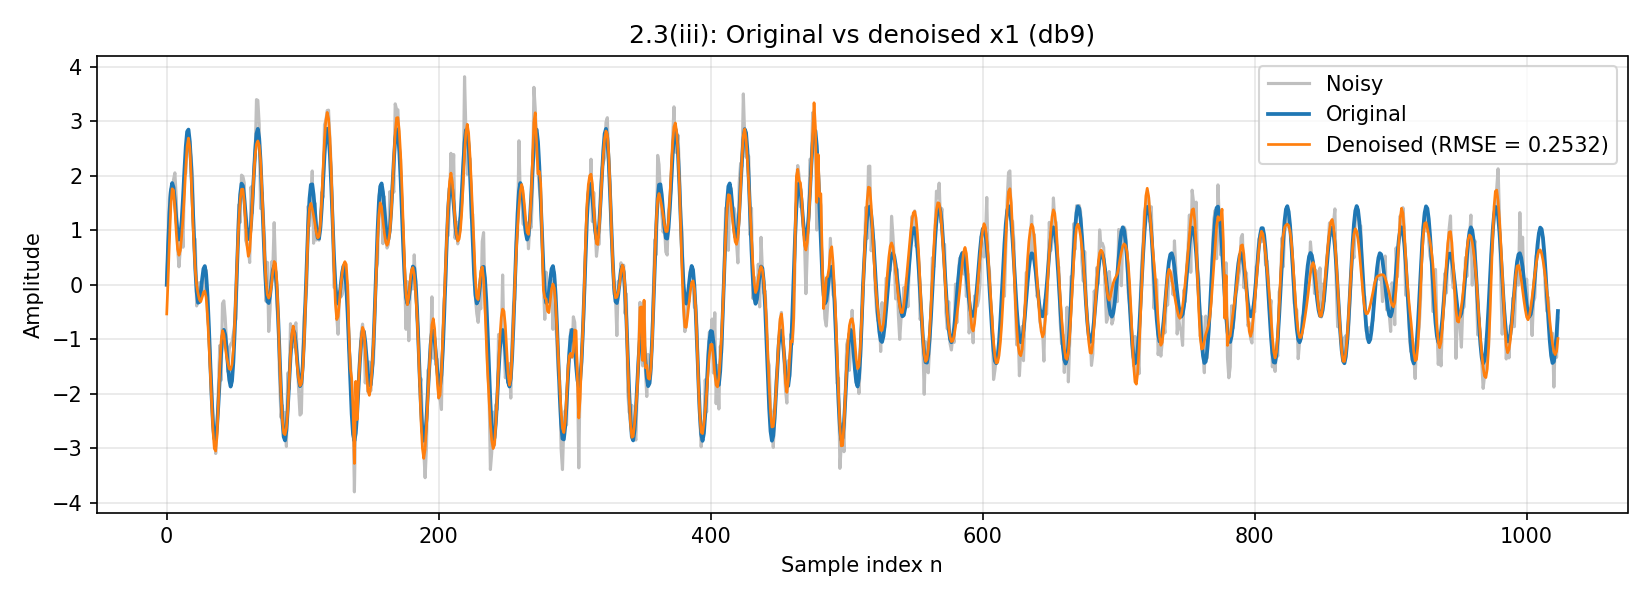
\includegraphics[width=\textwidth]{fig2_3_iii_denoised_x1_db9.png}
        \caption{$x_1$, db9}
    \end{subfigure}
    \begin{subfigure}{0.49\textwidth}
        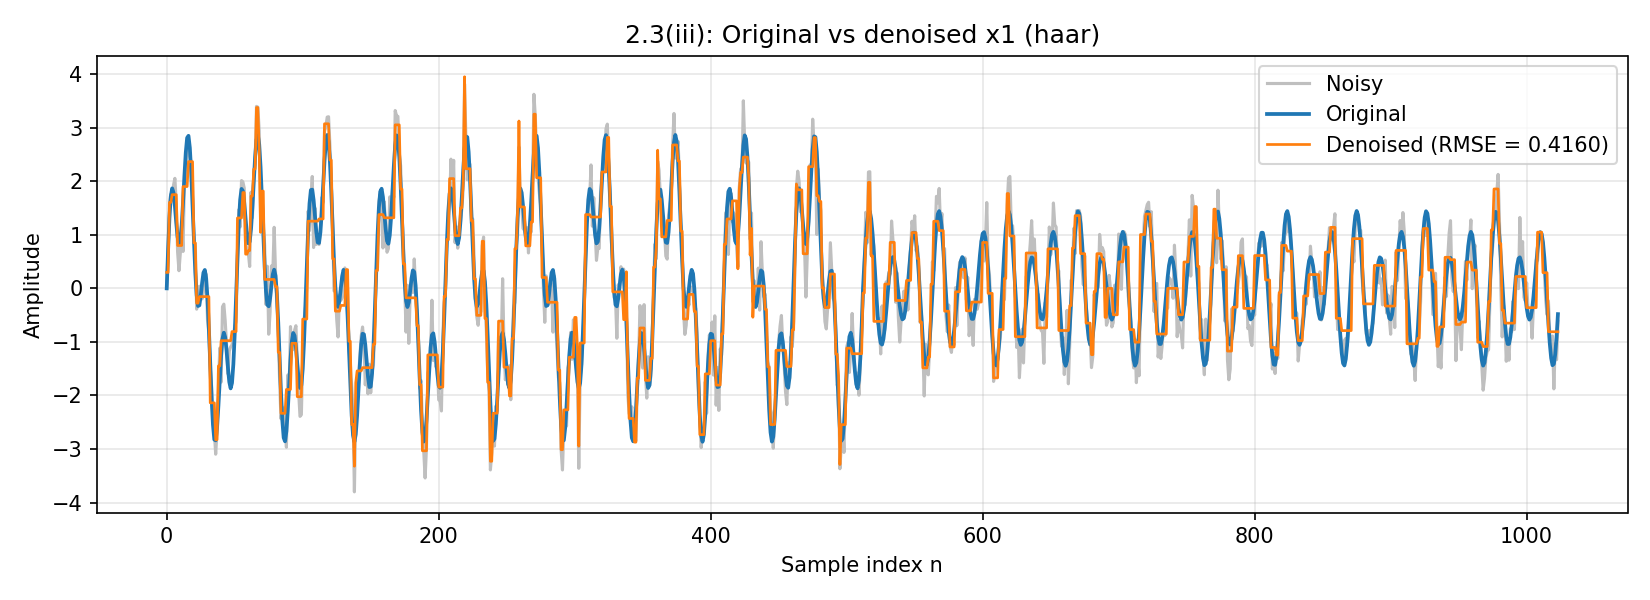
\includegraphics[width=\textwidth]{fig2_3_iii_denoised_x1_haar.png}
        \caption{$x_1$, Haar}
    \end{subfigure}
    \begin{subfigure}{0.49\textwidth}
        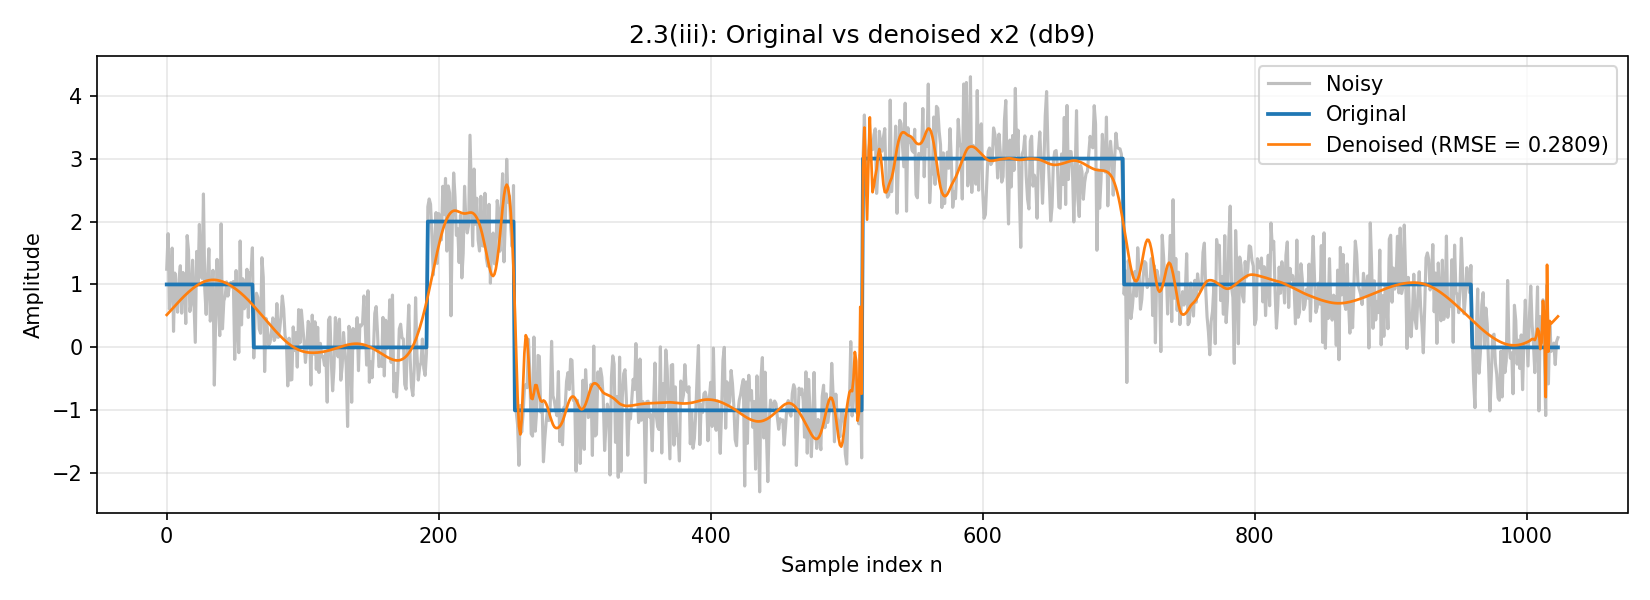
\includegraphics[width=\textwidth]{fig2_3_iii_denoised_x2_db9.png}
        \caption{$x_2$, db9}
    \end{subfigure}
    \begin{subfigure}{0.49\textwidth}
        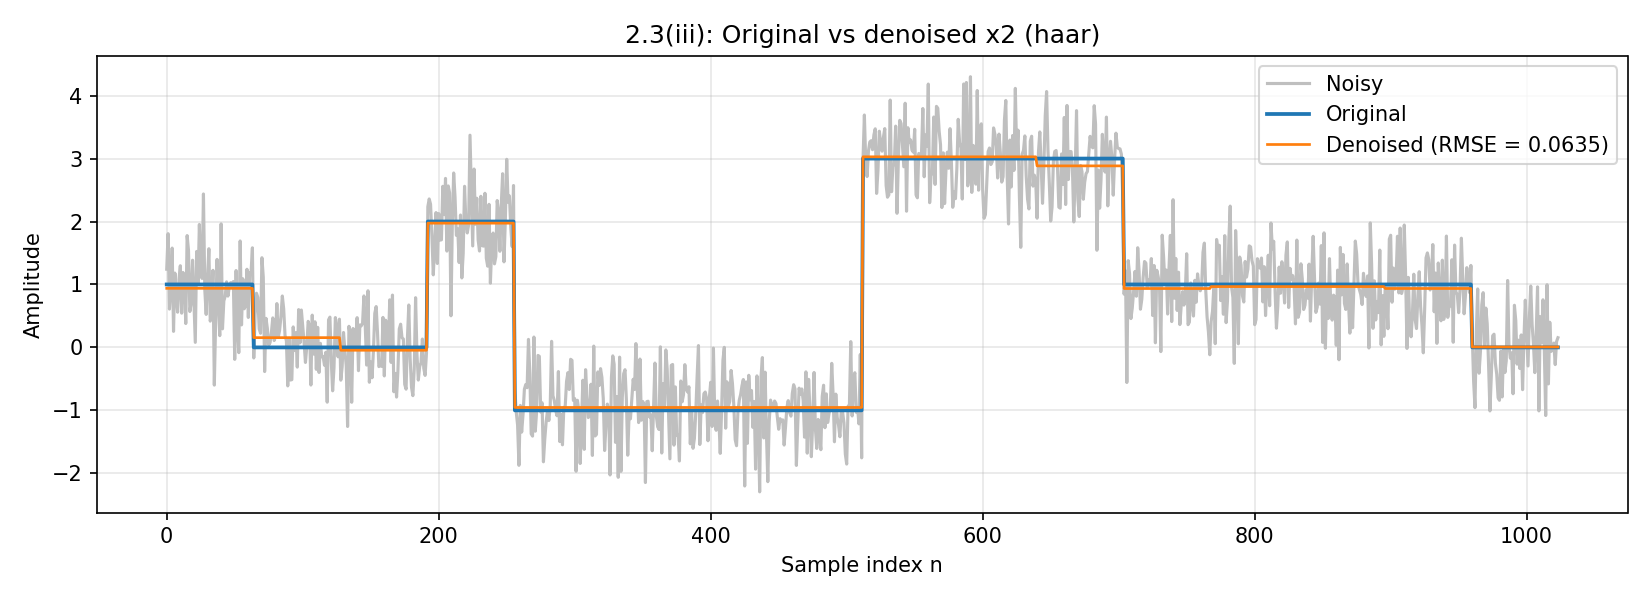
\includegraphics[width=\textwidth]{fig2_3_iii_denoised_x2_haar.png}
        \caption{$x_2$, Haar}
    \end{subfigure}
    \caption{Original, noisy and denoised signals.}
    \label{fig:denoised}
\end{figure}

With db9, the denoised $x_1$ follows the original sinusoids closely and the RMSE falls from 0.385 to 0.253; the remaining error is mainly a small amplitude loss at the peaks, since some weak signal coefficients are removed together with the noise. For $x_2$, db9 removes most of the noise on the flat segments (RMSE 0.515 to 0.281), but oscillations appear around every step.

\subsubsection*{(v) Comparison of db9 and Haar}

\begin{figure}[H]
    \centering
    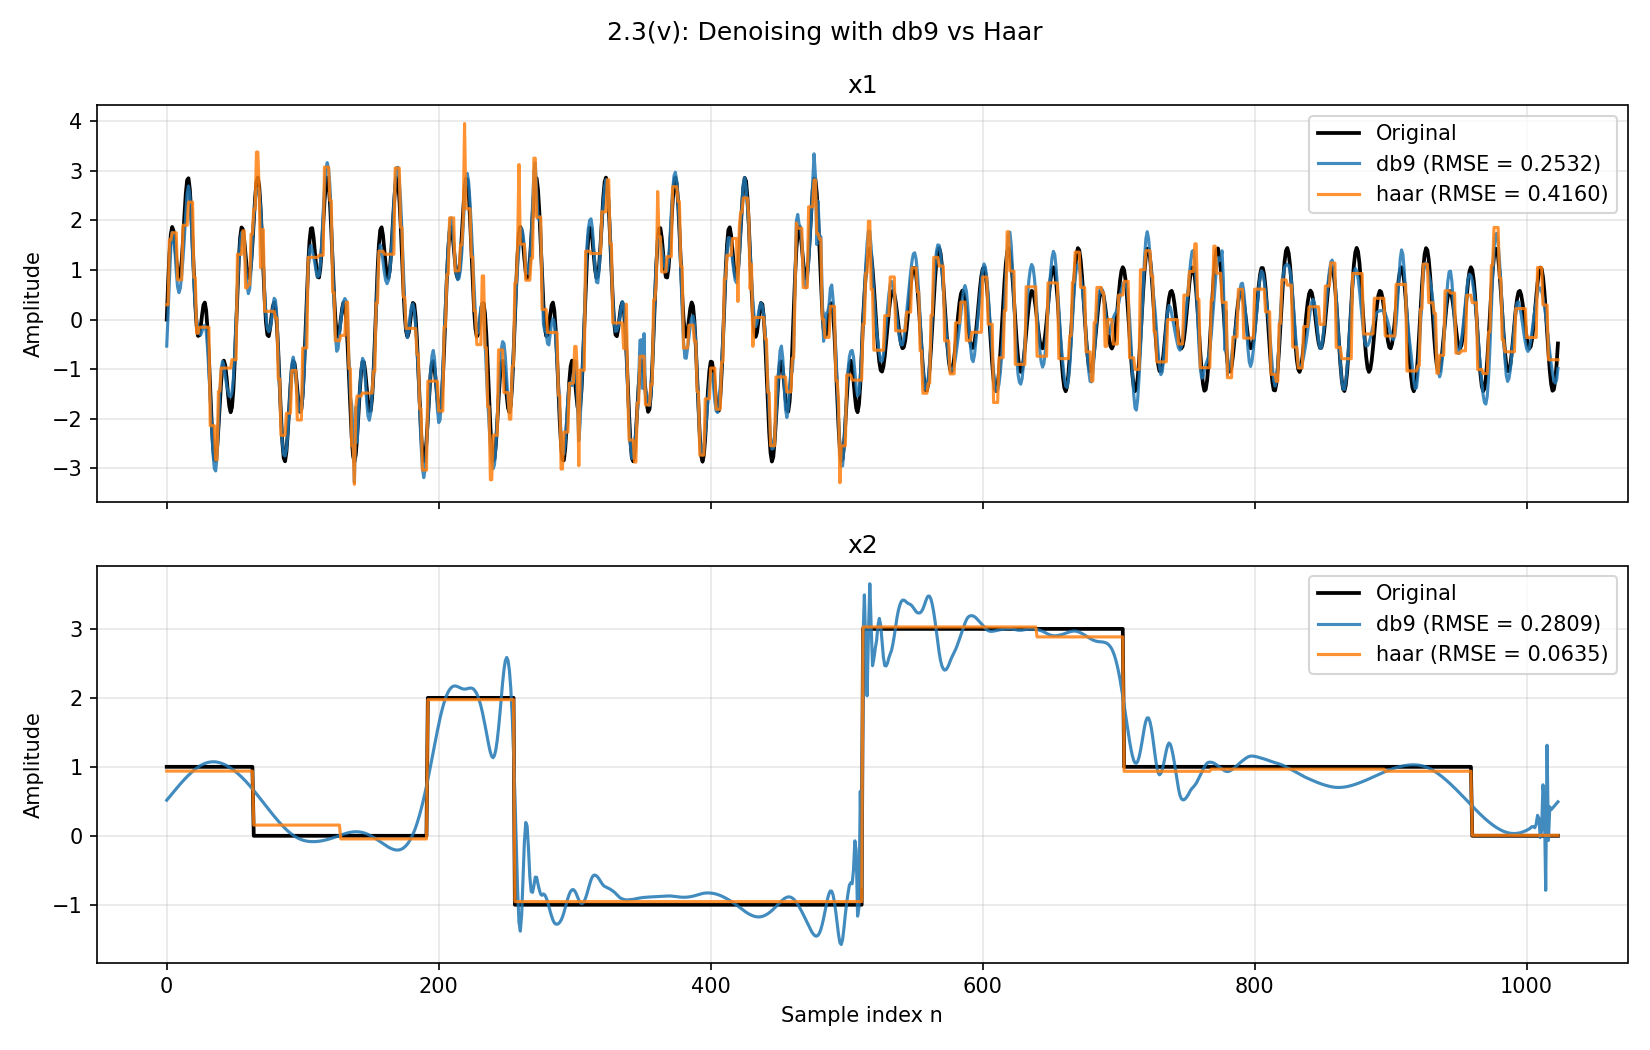
\includegraphics[width=0.9\textwidth]{fig2_3_v_db9_vs_haar.png}
    \caption{Denoised signals obtained with db9 and Haar compared with the originals.}
    \label{fig:compare}
\end{figure}

\begin{itemize}[leftmargin=*]
    \item \textbf{$x_1$ (smooth sinusoids): db9 is more suitable.} db9 gives a smooth reconstruction with an RMSE of 0.253. Haar gives a staircase-like waveform with spurious spikes and an RMSE of 0.416, which is higher than that of the noisy signal itself. A discontinuous wavelet needs many coefficients to approximate a smooth curve, so the signal energy is spread over many small coefficients that are not well separated from the noise: Haar keeps 219 coefficients and still performs worse than db9 with 154.
    \item \textbf{$x_2$ (piecewise constant): Haar is more suitable.} Haar reconstructs the steps almost exactly using only 11 coefficients (RMSE 0.064), because its basis functions have the same rectangular shape as the signal and the step positions lie on dyadic boundaries. db9 produces ringing (Gibbs-like oscillations) around every discontinuity and wrap-around artefacts at the signal ends, and gives an RMSE of 0.281 with 37 coefficients.
    \item \textbf{Conclusion.} Denoising performance depends on how sparsely the wavelet represents the signal. The best wavelet is the one whose shape resembles the signal: smooth wavelets with many vanishing moments (db9) for smooth, oscillatory signals, and Haar for signals with sharp edges and flat regions.
\end{itemize}

\subsection{Signal compression with the DWT}

\subsubsection*{(i) Wavelet coefficients of the ECG}

The aVR lead (2570 samples, $f_s = 257$~Hz, 10~s) was decomposed with db9 and Haar using the maximum useful level for each wavelet (level 7 for db9 and level 11 for Haar).

\subsubsection*{(ii) Coefficients required for 99\% of the energy}

The coefficients were sorted by magnitude in descending order and the cumulative sum of their squares was normalized by the total energy. $K$ is the smallest number of coefficients whose cumulative energy reaches 99\% (Figures~\ref{fig:energy_db9} and~\ref{fig:energy_haar}).

\begin{figure}[H]
    \centering
    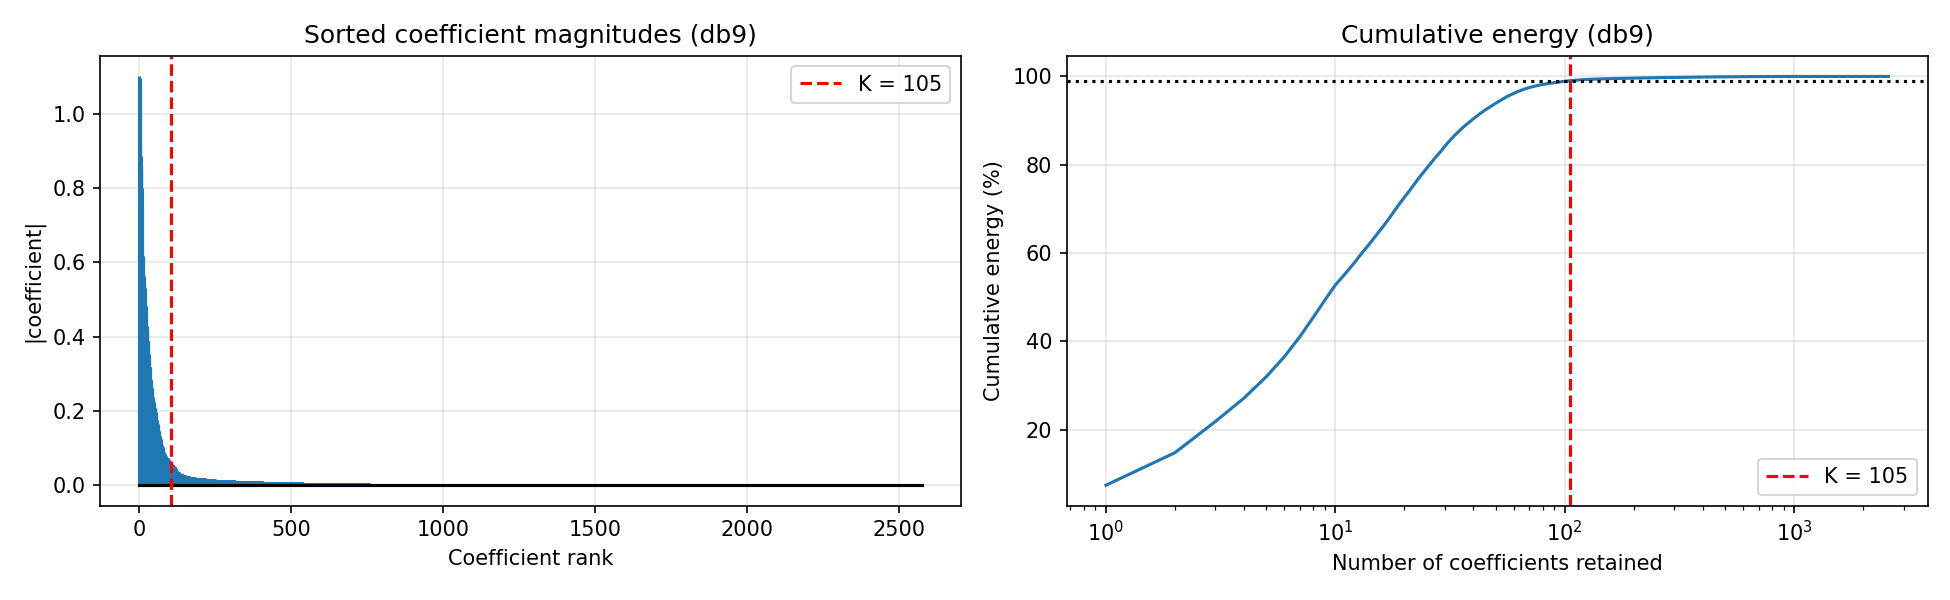
\includegraphics[width=0.9\textwidth]{fig2_4_ii_energy_db9.png}
    \caption{Sorted coefficient magnitudes and cumulative energy of the ECG (db9).}
    \label{fig:energy_db9}
\end{figure}

\begin{figure}[H]
    \centering
    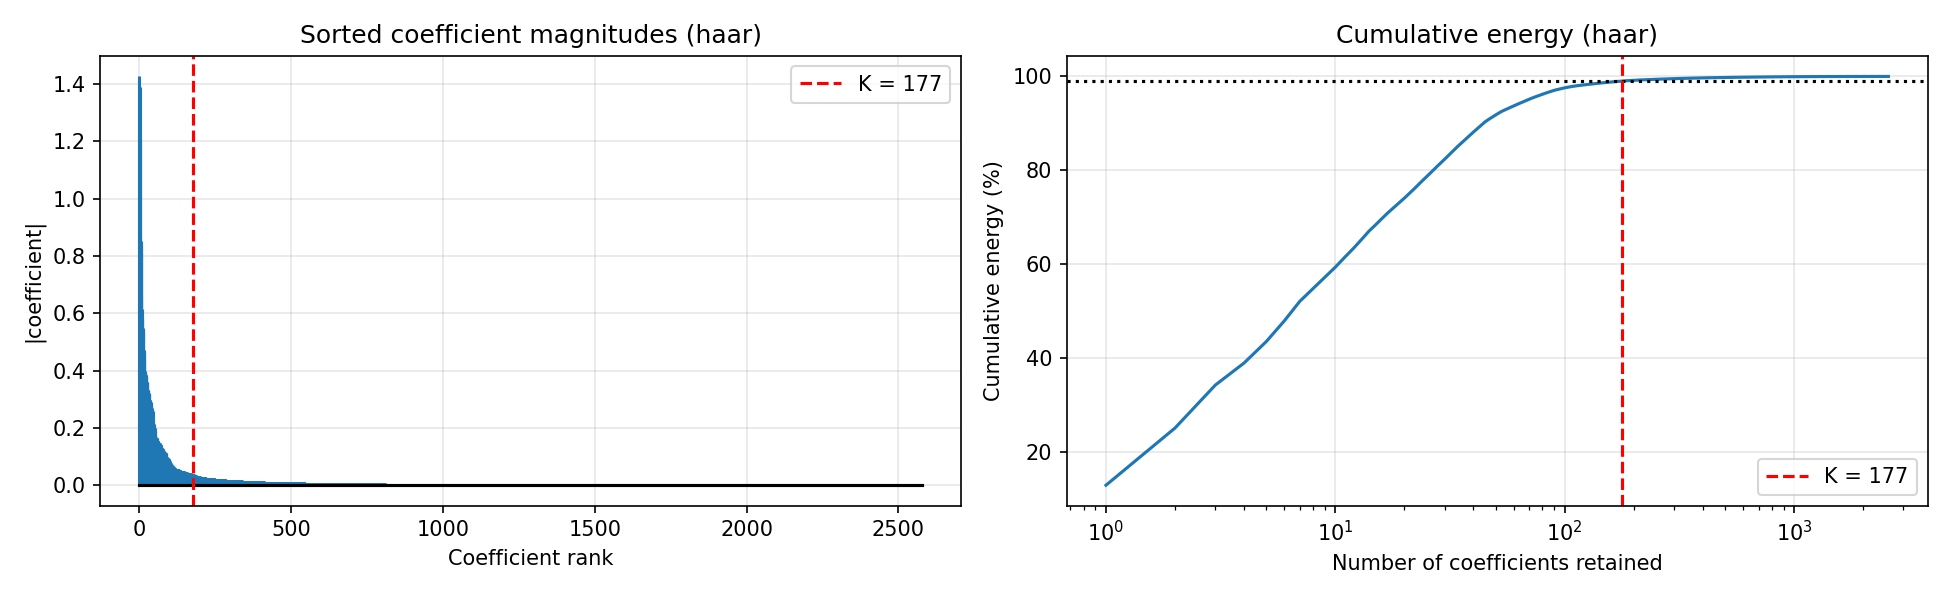
\includegraphics[width=0.9\textwidth]{fig2_4_ii_energy_haar.png}
    \caption{Sorted coefficient magnitudes and cumulative energy of the ECG (Haar).}
    \label{fig:energy_haar}
\end{figure}

\subsubsection*{(iii) Compression}

The signal was compressed by keeping the $K$ largest coefficients and setting the rest to zero, and then reconstructed with the inverse DWT. The compression ratio is defined as the number of samples of the original signal divided by the number of retained coefficients, $\mathrm{CR} = N/K$.

\begin{table}[H]
    \centering
    \begin{tabular}{lccccc}
        \toprule
        Wavelet & Level & Total coefficients & $K$ (99\% energy) & Compression ratio & RMSE \\
        \midrule
        db9  & 7  & 2575 & 105 & 24.48 : 1 & 0.00786 \\
        Haar & 11 & 2578 & 177 & 14.52 : 1 & 0.00782 \\
        \bottomrule
    \end{tabular}
    \caption{ECG compression results at 99\% retained energy ($N = 2570$).}
    \label{tab:compress}
\end{table}

\begin{figure}[H]
    \centering
    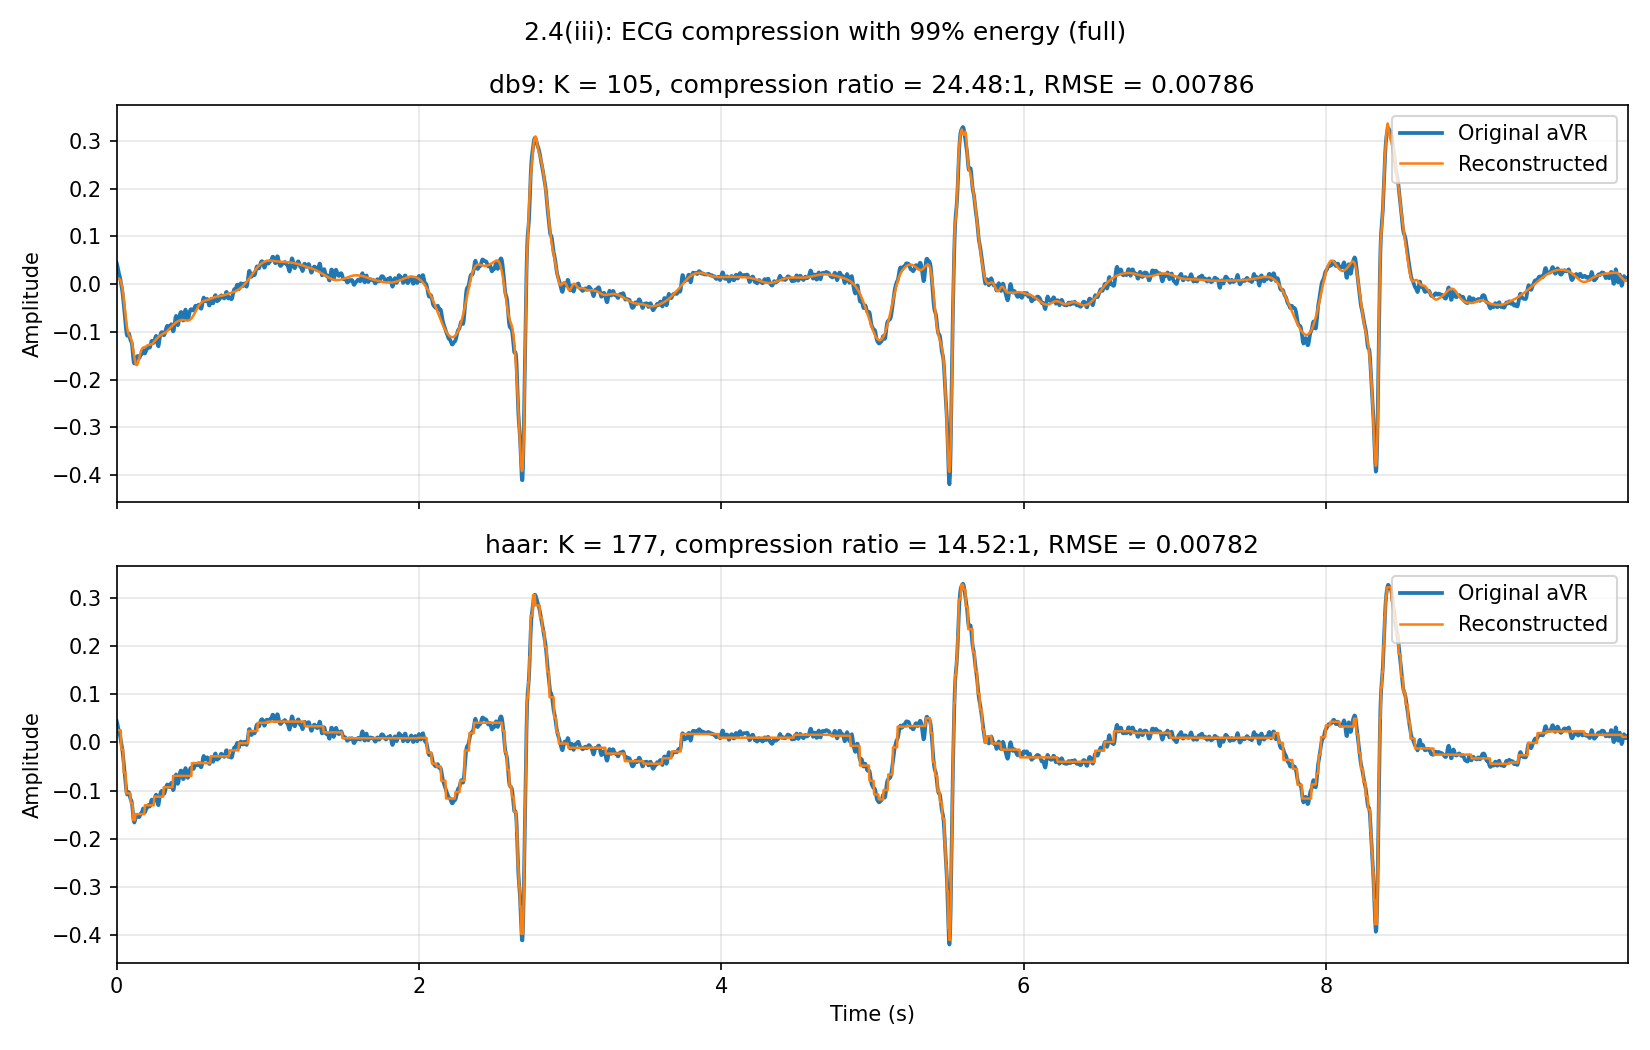
\includegraphics[width=0.9\textwidth]{fig2_4_iii_compressed_ecg_full.png}
    \caption{Original and reconstructed ECG (full record).}
    \label{fig:ecg_full}
\end{figure}

\begin{figure}[H]
    \centering
    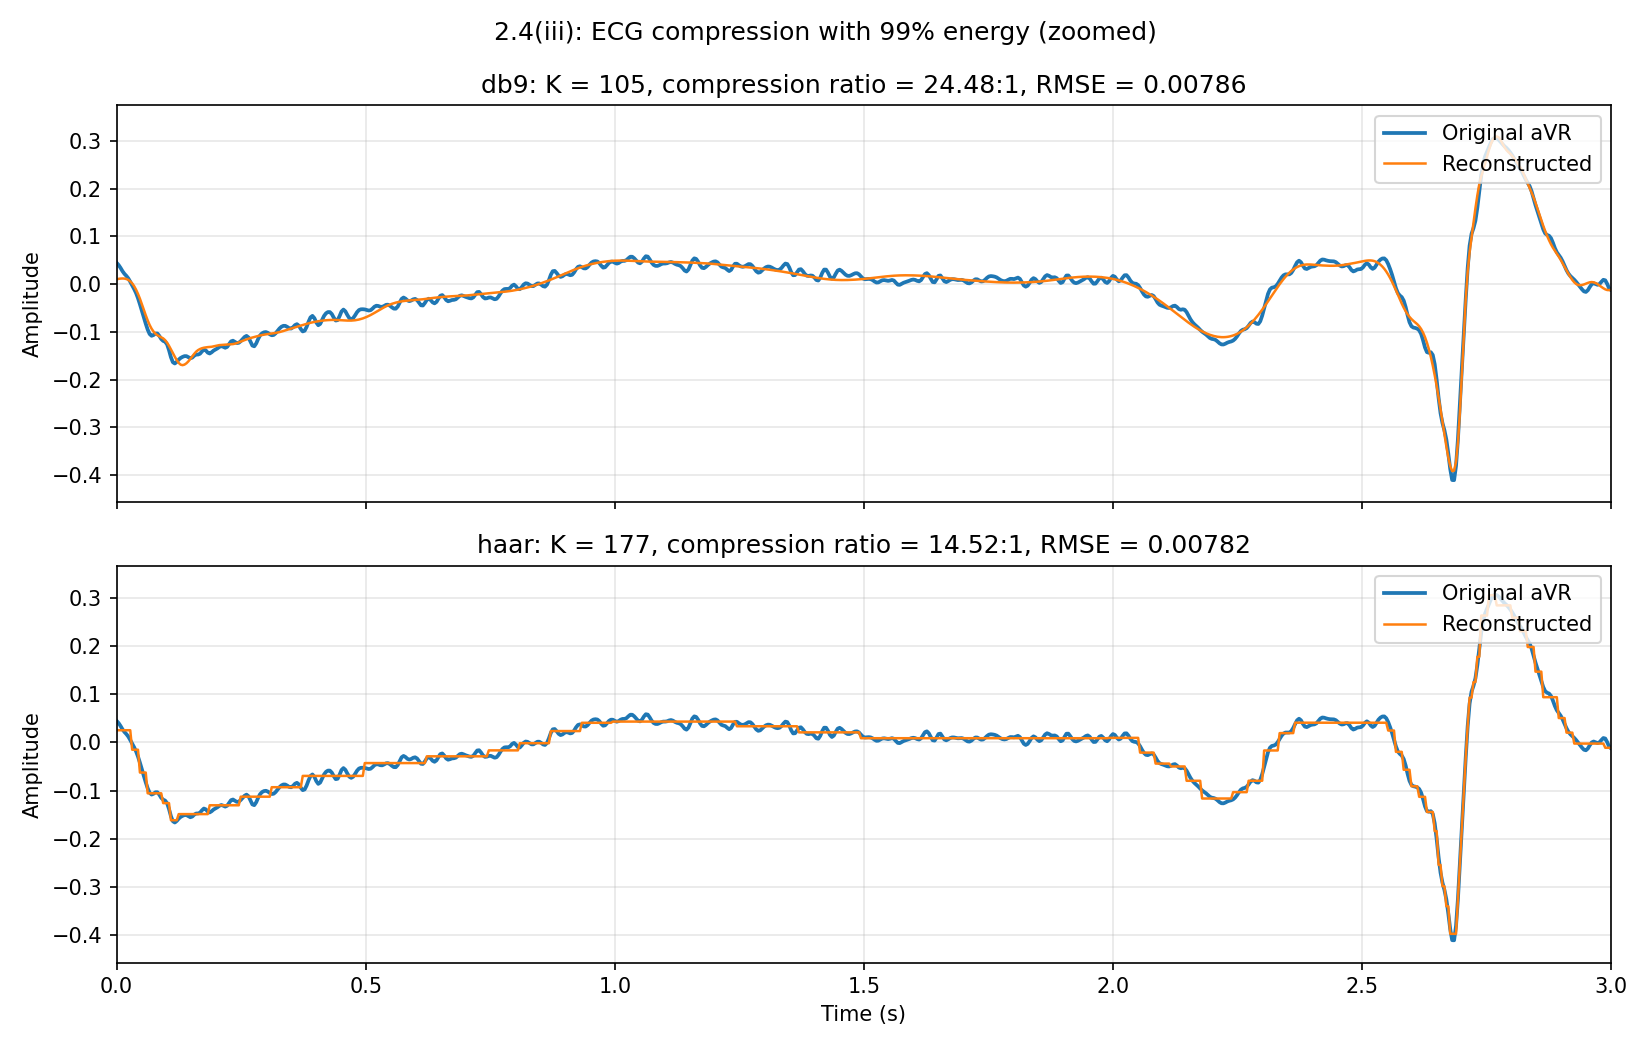
\includegraphics[width=0.9\textwidth]{fig2_4_iii_compressed_ecg_zoomed.png}
    \caption{Original and reconstructed ECG (first 3~s).}
    \label{fig:ecg_zoom}
\end{figure}

\begin{itemize}[leftmargin=*]
    \item \textbf{Compression ratio.} About 4\% of the coefficients are enough to hold 99\% of the energy with db9 (105 coefficients, 24.5:1), while Haar requires 177 coefficients (14.5:1). The ECG is a mostly smooth signal, so the smooth db9 wavelet with nine vanishing moments represents it more sparsely than the discontinuous Haar wavelet.
    \item \textbf{Error.} Since both reconstructions retain 99\% of the energy, the error is almost the same in both cases (RMSE $\approx 0.0078$, which corresponds to a percentage RMS difference of about 10\%). The difference between the wavelets lies in how many coefficients are needed and in the shape of the error.
    \item \textbf{Morphology with db9.} The reconstructed waveform is smooth and follows the baseline, the P and T waves and the QRS complex closely, with the QRS amplitude and timing preserved. The small high-frequency ripple on the original signal is removed, since it carries little energy; the compression therefore also acts as a denoiser.
    \item \textbf{Morphology with Haar.} The main features and the QRS complex are also preserved, but the slowly varying segments are reconstructed as a staircase (blocking artefacts), which is not physiological and could affect the interpretation of low-amplitude features such as the P wave and the ST segment.
    \item \textbf{Conclusion.} db9 is the more suitable wavelet for ECG compression: it gives a higher compression ratio at the same retained energy and a reconstruction that is visually much closer to a real ECG.
\end{itemize}

\end{document}
